\documentclass[12pt,a4paper,oneside]{book}
\usepackage[utf8]{vietnam}
\usepackage{amsmath,amsfonts,amssymb}
\usepackage{graphicx}
\usepackage[top=1.5cm, bottom=2cm, left=2cm, right=1.5cm]{geometry}
\usepackage{tikz}   
\usetikzlibrary{angles,calc}
\usepackage[table]{xcolor}
\usepackage{tcolorbox}  
\tcbuselibrary{breakable,most,many,skins}
\usepackage{fontawesome}
\usepackage[loigiai]{style/ex_test}
\usepackage{style/set_box}
\usepackage{varwidth}
\usepackage[version=4]{mhchem}
\usepackage{needspace}
\usepackage{pdfpages}

\usepackage{paracol} % Gói lệnh chia cột song song
\columnratio{0.5}    % Tỷ lệ 2 cột (0.5 là mỗi bên 50%)
\globalcounter{paragraph}
\setlength{\columnseprule}{1pt}

\def\sbHD{}
\newcommand{\doicot}{\switchcolumn\sbHD}

%---- Cài đặt màu mặc định gói set_box ----
\setboxColframeSetDefault{black}
\setboxColbackSetDefault{black!5}
\setboxColbacktitleSetDefault{brown!30}
\theoremstyle{immini}

% Kiến thức trọng tâm
\newtheorem{kttt}{Kiến thức trọng tâm}
\setTheoBox{kttt}{15}
\newtheorem{chuy}{Chú ý}
\setTheoBox*{chuy}{24}
\newtheorem{nhanxet}{Nhận xét}
\setTheoBox*{nhanxet}{22}

% Tình huống gợi vấn đề
\newenvironment{thgvd}{%
	\def\sbHD{\noindent\faBookmarkO~\textit{\textbf{Mở đầu:}}\par}
	\begin{paracol}{2}%
	\sbHD%
}{%
	\end{paracol}
}

% Tìm tòi - Khám phá
\newenvironment{ttkp}{%
	\def\sbHD{\noindent\faBookmarkO~\textit{\textbf{Tìm tòi - Khám phá:}}\par}
	\begin{paracol}{2}%
	\sbHD%
	}{%
	\end{paracol}
}

% Đọc hiểu - Nghe hiểu
\newenvironment{dhnh}{%
	\def\sbHD{\noindent\faBookmarkO~\textit{\textbf{Đọc hiểu - Nghe hiểu:}}\par}
	\begin{paracol}{2}%
		\sbHD%
	}{%
	\end{paracol}
}

% Ví dụ
\newcounter{vidu}
\newenvironment{vidu}{%
	\refstepcounter{vidu}
	\def\sbHD{\noindent\faBookmarkO~\textit{\textbf{Ví dụ \thevidu:}}\par}
	\begin{paracol}{2}%
	\sbHD%
	}{%
	\end{paracol}
}

% Luyện tập
\newcounter{luyentap}
\newenvironment{luyentap}{%
	\refstepcounter{luyentap}
	\def\sbHD{\noindent\faBookmarkO~\textit{\textbf{Luyện tập \theluyentap:}}\par}
	\begin{paracol}{2}%
	\sbHD%
	}{%
	\end{paracol}
}

% Tổ chức thực hiện
\newenvironment{tcth}{%
	\begin{itemize}
}{%
	\end{itemize}
}
\newcommand{\buocmot}{\item[]\hspace{-\leftmargin}\textbf{Bước 1.} Giao nhiệm vụ học tập}
\newcommand{\buochai}{\item[]\hspace{-\leftmargin}\textbf{Bước 2.} Thực hiện nhiệm vụ}
\newcommand{\buocba}{\item[]\hspace{-\leftmargin}\textbf{Bước 3.} Báo cáo, thảo luận}
\newcommand{\buocbon}{\item[]\hspace{-\leftmargin}\textbf{Bước 4.} Kết luận, nhận định}

\usepackage{titletoc}
\usepackage[explicit]{titlesec}

\setcounter{secnumdepth}{5}
\setcounter{tocdepth}{3}

% Chương
\titleformat{\chapter}
{\normalfont\bf\Huge}
{}
{0em}
{\ifthenelse{\equal{\thechapter}{0}}{#1}{\chaptername~\thechapter\\[0.6cm]#1}}
[\ifthenelse{\equal{\thechapter}{0}}{}{\vfill\clearpage}]

% Bải dạy
\titlespacing{\section}{0mm}{0mm}{0mm}[0mm]
\titleformat{\section}
{\normalfont}
{}
{0em}
{%
	\needspace{6\baselineskip}%
	\begin{tcolorbox}[colback=white, colframe=black, boxrule=1pt, before skip=0pt, after skip=0pt, top=2mm, bottom=2mm]
	    % Chia làm 2 cột bằng minipage
	    \begin{minipage}[t]{0.45\textwidth}
	        \textbf{Trường: \truong}\\
	        \textbf{Tổ: \tobomon}
	    \end{minipage}
	    \hfill
	    \begin{minipage}[t]{0.45\textwidth}
	        \centering
	        Họ và tên giáo viên:\\
	        \giaovien
	    \end{minipage}
	    \vspace{0.3cm} % Khoảng cách dòng
	    \begin{center}
	        \textbf{TÊN BÀI DẠY: #1}\\[0.3cm]
	        Môn học/Hoạt động giáo dục: \monhoc; lớp: \lophoc\\
			Thời gian thực hiện: \thoigian~(tiết)
	    \end{center}
	\end{tcolorbox}
}

% Mục lớn (mục tiêu, thiết bị dạy học, tiến trình dạy học, phụ lục...)
\titlespacing{\subsection}{0mm}{2mm}{2mm}[0mm]
\titleformat{\subsection}
{\normalfont\bf}
{\Roman{subsection}.}
{0.5em}
{\MakeUppercase{#1}}

% Tiết (1, 2, 3,...)
\titlespacing{\subsubsection}{0mm}{0mm}{0mm}[0mm]
\titleformat{\subsubsection}[block]
{\normalfont\bf}
{}
{0em}
{%
	\needspace{6\baselineskip}%
	\begin{tcolorbox}[colback=white, colframe=black, boxrule=1pt, before skip=0pt, after skip=0pt, top=2mm, bottom=2mm]
		\hfil\bf Tiết \arabic{subsubsection}. #1%
	\end{tcolorbox}
}

% Hoạt động (mở đầu, hình thành kiến thức, luyện tập, vận dụng)
\titlespacing{\paragraph}{0mm}{2mm}{2mm}[0mm]
\titleformat{\paragraph}[block]
{\normalfont\bf}
{\arabic{paragraph}.}
{0.5em}
{#1}

% Các phần của hoạt động (mục tiêu, nội dung, sản phẩm, tổ chức thực hiện)
\titlespacing{\subparagraph}{0mm}{0mm}{0mm}[0mm]
\titleformat{\subparagraph}[block]
{\normalfont\bf}
{\alph{subparagraph})}
{0.5em}
{#1}
\usepackage[hidelinks]{hyperref}
\usepackage{titletoc}

\setcounter{tocdepth}{3}

% Mục lục
\renewcommand{\contentsname}{MỤC LỤC}

% Chương
\titlecontents{chapter}[0mm]
{%
    \bf
    \ifthenelse{\equal{\thecontentslabel}{}}{%
    }{%
        Chương~\thecontentslabel.
    }
}
{}
{}
{\hfill\contentspage}

% Bải dạy
\titlecontents{section}[7mm]
{%
    \faCaretRight~\bf
    %%% \section không đánh số thì sẽ không in Bài 
    % \ifthenelse{\equal{\thecontentslabel}{}}{%
    % }{%
    %     Bài~\thecontentslabel.
    % }
}
{}
{}
{\titlerule*[0.3pc]{.}\quad\contentspage}

% Mục lớn (mục tiêu, thiết bị dạy học, tiến trình dạy học, phụ lục...)
\titlecontents{subsection}[14mm]
{%
    \ifthenelse{\equal{\thecontentslabel}{}}{%
    }{%
        \thecontentslabel.
    }
}
{}
{}
{\titlerule*[0.3pc]{.}\quad\contentspage}

% Tiết (1, 2, 3,...)
\titlecontents{subsubsection}[21mm]
{%
    \ifthenelse{\equal{\thecontentslabel}{}}{%
    }{%
        Tiết~\thecontentslabel.
    }
}
{}
{}
{\titlerule*[0.3pc]{.}\quad\contentspage}

\newcommand{\hoac}[1]{\left[\begin{aligned}#1\end{aligned}\right.}
\newcommand{\heva}[1]{\left\{\begin{aligned}#1\end{aligned}\right.}

\newcommand{\thoai}[1]{{\it #1}}

%%% Tên bài học
\def\truong{THCS XXX}
\def\tobomon{Toán}
\def\giaovien{Phan Văn Anh}
\def\monhoc{Toán}
\def\lophoc{9AX}

%%% Tất biểu tượng
% \tatBieuTuong

\begin{document}
	% Bìa
	\thispagestyle{empty}
	
\includepdf{cover/cover.pdf}
	% Mục lục
	\pagestyle{plain}
	\tableofcontents
	%
	\chapter
	[PHƯƠNG TRÌNH VÀ HỆ PHƯƠNG TRÌNH BẬC NHẤT HAI ẨN]
	{PHƯƠNG TRÌNH VÀ HỆ PHƯƠNG TRÌNH BẬC NHẤT HAI ẨN}
	%
	\input{data/9D1-1}
	\newpage
	\def\thoigian{4}
\section
[Giải hệ hai phương trình bậc nhất hai ẩn]
{GIẢI HỆ HAI PHƯƠNG TRÌNH BẬC NHẤT HAI ẨN}

\subsection{Mục tiêu}

\paragraph{Về kiến thức, kĩ năng}

\begin{itemize}
    \item Giải hệ hai phương trình bậc nhất hai ẩn bằng phương pháp thế và phương pháp cộng đại số. 
    \item Tìm nghiệm của hệ hai phương trình bậc nhất hai ẩn bằng máy tính cầm tay (MTCT). 
\end{itemize}

\paragraph{Về năng lực}

\begin{itemize}
    \item Rèn luyện các năng lực toán học, nói riêng là năng lực tư duy và lập luận toán học, năng lực sử dụng công cụ và phương tiện học toán. 
    \item Bồi dưỡng hứng thú học tập, ý thức làm việc nhóm, ý thức tìm tòi, khám phá và sáng tạo cho HS. 
\end{itemize}

\paragraph{Về phẩm chất}

\begin{itemize}
    \item Góp phần giúp HS rèn luyện và phát triển các phẩm chất tốt đẹp (yêu nước, nhân ái, chăm chỉ, trung thực, trách nhiệm):
    \begin{itemize}
        \item Tích cực phát biểu, xây dựng bài và tham gia các hoạt động nhóm;
        \item Có ý thức tích cực tìm tòi, sáng tạo trong học tập; phát huy điểm mạnh, khắc phục các điểm yếu của bản thân. 
    \end{itemize}
\end{itemize}

\subsection{Thiết bị dạy học và học liệu}

\paragraph{Giáo viên}

\begin{itemize}
    \item Giáo án, bảng phụ, máy chiếu (nếu có), phiếu học tập, … 
\end{itemize}

\paragraph{Học sinh}

\begin{itemize}
    \item SGK, vở ghi, dụng cụ học tập, máy tính cầm tay. 
\end{itemize}

\subsection{Tiến trình dạy học}

Bài học này dạy trong 04 tiết: 
\begin{itemize}
    \item Tiết 1: Mục 1. Phương pháp thế.
    \item Tiết 2: Mục 2. Phương pháp cộng đại số.
    \item Tiết 3: Mục 3. Sử dụng MTCT tìm nghiệm của hệ hai phương trình bậc nhất hai ẩn.
    \item Tiết 4: Chữa bài tập. 
\end{itemize}

\subsubsection{Phương pháp thế}

\paragraph{Hoạt động khởi động}

\muctieu

\begin{itemize}
    \item Gợi động cơ, tạo tình huống có vấn đề về việc giải hệ hai phương trình bậc nhất hai ẩn. 
\end{itemize}

\noidungsanpham

\begin{modau}
    Một mảnh vườn được đánh thành nhiều luống, mỗi luống trồng cùng một số cây cải bắp. Hãy tính số cây cải bắp được trồng trên mảnh vườn đó, biết rằng:
    \begin{itemize}
    \item Nếu tăng thêm 8 luống, nhưng mỗi luống trồng ít đi 3 cây cải bắp thì số cải bắp của cả vườn sẽ ít đi 108 cây;
    \item Nếu giảm đi 4 luống, nhưng mỗi luống trồng tăng thêm 2 cây thì số cải bắp cả vườn sẽ tăng thêm 64 cây.
    \end{itemize}
\end{modau}

\tochucthuchien

\begin{tcth}
    \buocmot
    \item GV yêu cầu HS đọc nội dung của Tình huống mở đầu. 
    \buochai
    \item HS suy nghĩ về tình huống mở đầu và nảy sinh nhu cầu tìm hiểu cách giải hệ hai phương trình bậc nhất hai ẩn.
    \buocba
    \item HS trả lời câu hỏi (không yêu cầu trả lời chính xác).
    \buocbon
    \item GV giới thiệu bài học mới về giải phương trình bậc nhất hai ẩn.
\end{tcth}

\paragraph{Hoạt động hình thành kiến thức}

\muctieu

\begin{itemize}
    \item HS biết cách giải hệ hai phương trình bậc nhất hai ẩn bằng phương pháp thế. 
\end{itemize}

\noidungsanpham

\begin{ttkp}
    \textbf{Làm quen với phương pháp thế}\\
    \textbf{HĐ1:} 
    Cho hệ phương trình $\heva{&x+y=3\\&2x-3y=1}$. Giải hệ phương trình theo hướng dẫn sau:
    \begin{listEX} 
        \item Từ phương trình thứ nhất, biểu diễn y theo x rồi thế vào phương trình thứ hai để được một phương trình với một ẩn x. Giải phương trình một ẩn đó để tìm giá trị của x. 
        \item Sử dụng giá trị tìm được của x để tìm giá trị của y rồi viết nghiệm của hệ phương trình đã cho. 
    \end{listEX}
    %%%
    \doicot
    %%%
    \textbf{HĐ1:}
    \begin{listEX}
        \item Từ phương trình thứ nhất, ta có $x=3-y$.\\
        Thế vào phương trình thứ hai ta được $2(3-y)-3y=1$, suy ra $y=1$.
        \item Với $y=1$ thì $x=3-1=2$.\\
        Vậy nghiệm của hệ đã cho là $(2;1)$.
    \end{listEX} 
\end{ttkp}

\begin{vidu}
    Giải hệ phương trình $\heva{&2x-y=3\\&x+2y=4}$ bằng phương pháp thế.
    %%%
    \doicot
    %%%
    Từ phương trình thứ nhất của hệ ta có $y = 2x - 3$. Thế vào phương trình thứ hai của hệ, ta được $x + 2(2x - 3) = 4$ hay $5x - 6 = 4$, suy ra $x = 2$.\\
    Từ đó $y = 2 \cdot 2 - 3 = 1$. Vậy hệ phương trình đã cho có nghiệm là $(2; 1)$.
\end{vidu}

\tochucthuchien

\begin{tcth}[ttkp]
    \buocmot
    \item GV hướng dẫn HS thực hiện lần lượt các yêu cầu trong HĐ1.
    \buochai
    \item HS thực hiện cá nhân HĐ1. 
    \buocba
    \item GV yêu cầu HS nêu cách giải hệ phương trình bậc nhất hai ẩn bằng phương pháp thế.
    \item HS giơ tay phát biểu.
    \buocbon
    \item GV nhận xét, kết luận và phân tích cách giải hệ phương trình bằng phương pháp thế.
    \item GV viết bảng hoặc trình chiếu nội dung trong Khung kiến thức. 
    \begin{kttt}
        \textbf{Cách giải hệ phương trình bằng phương pháp thế:}
        \begin{cacbuoc}
            \item Từ một phương trình của hệ, biểu diễn một ẩn theo ẩn kia rồi thế vào phương trình còn lại của hệ để được phương trình chỉ còn chứa một ẩn.
            \item Giải phương trình một ẩn vừa nhận được, từ đó suy ra nghiệm của hệ đã cho.
        \end{cacbuoc}
    \end{kttt}
\end{tcth}

\begin{tcth}[vidu=1]
    \buocmot
    \item GV yêu cầu HS hoạt động cá nhân trong 3 phút để giải hệ phương trình của Ví dụ 1 bằng phương pháp thế.
    \buochai
    \item HS thực hiện theo hướng dẫn của GV.
    \buocba
    \item HS giơ tay phát biểu.
    \buocbon
    \item GV chữa bài và hướng dẫn chi tiết các bước làm cho HS.
\end{tcth}

\paragraph{Hoạt động luyện tập}

\muctieu

\begin{itemize}
    \item Củng cố kĩ năng giải hệ hai phương trình bậc nhất hai ẩn bằng phương pháp thế.
\end{itemize}

\noidungsanpham

\begin{luyentap}
    Giải các hệ phương trình sau bằng phương pháp thế:
    \begin{listEX}
        \item $\heva{&x - 3y = 2 \\ &-2x + 5y = 1}$;
        \item $\heva{&4x + y = -1 \\ &7x + 2y = -3}$.
    \end{listEX}
    %%%
    \doicot
    %%%
    \huongdan
    \begin{listEX}
        \item Kết quả là $(-13 ; -5)$.\\
        Tình huống biểu diễn $x$ theo $y$; 
        \item Kết quả là $(1 ; -5)$.\\
        Tình huống biểu diễn $y$ theo $x$. 
    \end{listEX}
\end{luyentap}

\begin{vidu}
    Giải hệ phương trình $\heva{&x - y = -2 \\ &2x - 2y = 8}$ bằng phương pháp thế.
    %%%
    \doicot
    %%%
    Từ phương trình thứ nhất ta có $x = y - 2$. Thế vào phương trình thứ hai, ta được $2(y - 2) - 2y = 8$ hay $0y - 4 = 8$. \quad (1)\\
    Do không có giá trị nào của $y$ thoả mãn hệ thức (1) nên hệ phương trình đã cho vô nghiệm.
\end{vidu}

\begin{luyentap}
    Giải hệ phương trình $\heva{&-2x + y = 3 \\ &4x - 2y = -4}$ bằng phương pháp thế.
    %%%
    \doicot
    %%%
    \huongdan\\
    Biểu diễn $y$ theo $x$ từ phương trình thứ nhất, kết quả hệ vô nghiệm.
\end{luyentap}

\begin{vidu}
    Giải hệ phương trình $\heva{&-x + y = -2 \\ &3x - 3y = 6}$ bằng phương pháp thế.
    %%%
    \doicot
    %%%
    Từ phương trình thứ nhất ta có $y = x - 2$. \quad (2)\\
    Thế vào phương trình thứ hai, ta được $3x - 3(x - 2) = 6$ hay $0x = 0$. \quad (3)\\
    Ta thấy mọi giá trị của $x$ đều thoả mãn hệ thức (3).\\
    Với giá trị tuỳ ý của $x$, giá trị tương ứng của $y$ được tính bởi (2).\\
    Vậy hệ phương trình đã cho có nghiệm là $(x; x - 2)$ với $x \in \mathbb{R}$ tuỳ ý.
\end{vidu}

\begin{luyentap}
    Giải hệ phương trình $\heva{&x + 3y = -1 \\ &3x + 9y = -3}$ bằng phương pháp thế.
    %%%
    \doicot
    %%%
    \huongdan\\
    Hệ có nghiệm là $\left(x;\dfrac{-x-1}{3}\right)$, với $x\in\mathbb{R}$ tuỳ ý.
\end{luyentap}

\tochucthuchien

\begin{tcth}[luyentap=1]
    \buocmot
    \item GV yêu cầu HS làm việc cá nhân trong 4 phút.
    \item GV cần lưu ý cho HS, có thể chọn cách biểu diễn $x$ theo $y$ hoặc biểu diễn $y$ theo $x$. 
    \buochai
    \item HS thực hiện cá nhân Luyện tập 1. 
    \buocba
    \item GV gọi hai HS lên bảng trình bày lời giải.
    \buocbon
    \item GV chữa bài và hướng dẫn chi tiết các bước làm cho HS.
\end{tcth}

\begin{tcth}[vidu=2]
    \buocmot
    \item GV hướng dẫn HS thực hiện Ví dụ 2. 
    \item GV lưu ý cho HS: Nếu từ hệ đã cho, bằng phương pháp thế ta dẫn đến một phương trình vô nghiệm thì hệ đã cho vô nghiệm. 
    \buochai
    \item HS làm việc dưới sự hướng dẫn của GV. 
    \buocba
    \item HS làm bài vào vở.
    \buocbon
    \item GV chữa bài và hướng dẫn chi tiết các bước làm cho HS.
\end{tcth}

\begin{tcth}[luyentap=2]
    \buocmot
    \item GV yêu cầu HS làm việc cá nhân trong 3 phút.
    \buochai
    \item HS thực hiện cá nhân Luyện tập 2. 
    \buocba
    \item GV gọi HS lên bảng trình bày lời giải.
    \buocbon
    \item GV chữa bài và hướng dẫn chi tiết các bước làm cho HS.
\end{tcth}

\begin{tcth}[vidu=3]
    \buocmot
    \item GV hướng dẫn HS làm Ví dụ 3.
    \item GV lưu ý cho HS: Nếu từ hệ đã cho ta dẫn đến một phương trình nghiệm đúng với mọi $x$, $y$ thì hệ đã cho có vô số nghiệm. 
    \buochai
    \item HS làm việc dưới sự hướng dẫn của GV. 
    \buocba
    \item HS làm bài vào vở.
    \buocbon
    \item GV chữa bài và hướng dẫn chi tiết các bước làm cho HS.
\end{tcth}

\begin{tcth}[luyentap=3]
    \buocmot
    \item GV yêu cầu HS làm việc cá nhân thực hiện các câu của Luyện tập 3.  
    \buochai
    \item HS thực hiện cá nhân Luyện tập 3. 
    \buocba
    \item GV gọi HS lên bảng trình bày lời giải.
    \buocbon
    \item GV chữa bài và hướng dẫn chi tiết các bước làm cho HS.
\end{tcth}

\paragraph{Hoạt động vận dụng}

\muctieu

\begin{itemize}
    \item Giúp học sinh biết vận dụng kiến thức về hệ hai phương trình bậc nhất hai ẩn để trả lời câu hỏi của bài toán trong Tình huống mở đầu.
\end{itemize}

\noidungsanpham

\begin{vandung}
    Xét bài toán trong \textit{tình huống mở đầu}. Gọi $x$ là số luống trong vườn, $y$ là số cây cải bắp trồng ở mỗi luống ($x, y \in \mathbb{N}^*$).
    \begin{listEX}
        \item Lập hệ phương trình đối với hai ẩn $x$, $y$.
        \item Giải hệ phương trình nhận được ở câu a) để tìm câu trả lời cho bài toán.
    \end{listEX}
    %%%
    \doicot
    %%%
    \huongdan
    \begin{listEX}
        \item $\heva{&3x-8y=84\\&x-2y=36}$.
        \item Nghiệm của phương trình trên là $(60;12)$.\\
        Số cây bắp cải được trồng trên mảnh vườn đó là:
        $$60\cdot12=720\text{ (cây)}.$$
    \end{listEX}
\end{vandung}

\paragraph{Tổng kết và hướng dẫn công việc ở nhà}

GV tổng kết lại nội dung bài học và dặn dò công việc ở nhà cho HS:

\begin{itemize}
    \item  GV tổng kết lại các kiến thức trọng tâm của bài học: Cách giải hệ phương trình bằng phương pháp thế. 
    \item Nhắc HS về nhà ôn tập các nội dung đã học. 
    \item Giao cho HS làm bài tập trong SGK: Bài 1.6.
\end{itemize}

\subsubsection{Phương pháp cộng đại số}

\paragraph{Hoạt động hình thành kiến thức}

\muctieu

\begin{itemize}
    \item HS biết cách giải hệ hai phương trình bậc nhất hai ẩn bằng phương pháp cộng đại số. 
\end{itemize}

\noidungsanpham

\begin{ttkp}
    \textbf{HĐ2:}\\
    Cho hệ phương trình $\heva{&2x + 2y = 3 \\ &x - 2y = 6}$. Ta thấy hệ số của $y$ trong hai phương trình là hai số đối nhau (tổng của chúng bằng 0). Từ đặc điểm đó, hãy giải hệ phương trình đã cho theo hướng dẫn sau:
    \begin{listEX}
        \item Cộng từng vế của hai phương trình trong hệ để được phương trình một ẩn $x$. Giải phương trình này để tìm $x$.
        \item Sử dụng giá trị $x$ tìm được, thay vào một trong hai phương trình của hệ để tìm giá trị của $y$ rồi viết nghiệm của hệ phương trình đã cho.
    \end{listEX}
    %%%
    \doicot
    %%%
    \textbf{HĐ2:}\\
    \huongdan\\
    \begin{listEX}
        \item Cộng từng vế của hai phương trình ta được: $3x = 9$ nên $x = 3$.
        \item Với $x = 3$ ta có $3 - 2y = 6$ nên $y = \dfrac{-3}{2}$.\\
        Vậy nghiệm của hệ đã cho là $\left(3;\dfrac{-3}{2}\right)$.
    \end{listEX}
\end{ttkp}

\begin{vidu}
    Giải hệ phương trình $\heva{&-2x + 5y = 12 \\ &2x + 3y = 4}$ bằng \\
    phương pháp cộng đại số.
    %%%
    \doicot
    %%%
    Cộng từng vế hai phương trình ta được $8y = 16$, suy ra $y = 2$.\\
    Thế $y = 2$ vào phương trình thứ hai ta được $2x + 3 \cdot 2 = 4$, hay $2x = -2$, suy ra $x = -1$.\\
    Vậy hệ phương trình đã cho có nghiệm là $(-1; 2)$.
\end{vidu}

\begin{vidu}
    Giải hệ phương trình $\heva{&5x - 7y = 9 \\ &5x - 3y = 1}$ bằng phương pháp cộng đại số.
    %%%
    \doicot
    %%%
    Trừ từng vế của hai phương trình, ta được $(5x - 5x) + (-7y + 3y) = 9 - 1$ hay $-4y = 8$, suy ra $y = -2$.\\
    Thế $y = -2$ vào phương trình thứ nhất, ta được $5x - 7 \cdot (-2) = 9$ hay $5x + 14 = 9$, suy ra $x = -1$.\\
    Vậy hệ phương trình đã cho có nghiệm là $(-1; -2)$.
\end{vidu}

\tochucthuchien

\begin{tcth}[ttkp]
    \buocmot
    \item GV hướng dẫn HS thực hiện lần lượt các yêu cầu trong HĐ2.
    \buochai
    \item HS thực hiện cá nhân HĐ2.
    \buocba
    \item GV yêu cầu HS nêu cách giải hệ hai phương trình bậc nhất hai ẩn bằng phương pháp cộng đại số.
    \buocbon
    \item GV viết bảng hoặc trình chiếu nội dung trong Khung kiến thức.
    \begin{kttt}
        \textbf{Cách giải hệ phương trình bằng phương pháp cộng đại số:}\\
        Để giải một hệ hai phương trình bậc nhất hai ẩn có hệ số của cùng một ẩn nào đó trong hai phương trình bằng nhau hoặc đối nhau, ta có thể làm như sau:
        \begin{cacbuoc}
            \item Cộng hay trừ từng vế của hai phương trình trong hệ để được phương trình chỉ còn chứa một ẩn.
            \item Giải phương trình một ẩn vừa nhận được, từ đó suy ra nghiệm của hệ phương trình đã cho.
        \end{cacbuoc}
    \end{kttt}
\end{tcth}

\begin{tcth}[vidu=4]
    \buocmot
    \item GV hướng dẫn HS giải hệ phương trình của Ví dụ 4 bằng phương pháp cộng đại số.
    \item GV cần lưu ý cho HS trường hợp hệ số của $x$ đối nhau: Cộng từng vế hai phương trình.
    \buochai
    \item HS thực hiện dưới sự hướng dẫn của GV. 
    \buocba
    \item HS làm bài vào vở.
    \buocbon
    \item GV nhận xét, kết luận và phân tích cách giải hệ phương trình bằng phương pháp cộng đại số.
\end{tcth}

\begin{tcth}[vidu=5]
    \buocmot
    \item GV hướng dẫn HS giải hệ phương trình của Ví dụ 5 bằng phương pháp cộng đại số.
    \item GV cần lưu ý cho HS trường hợp hệ số của $x$ bằng nhau: Trừ từng vế hai phương trình.
    \buochai
    \item HS thực hiện dưới sự hướng dẫn của GV. 
    \buocba
    \item HS làm bài vào vở.
    \buocbon
    \item GV nhận xét, kết luận và phân tích cách giải hệ phương trình bằng phương pháp cộng đại số.
\end{tcth}

\paragraph{Hoạt động luyện tập}

\muctieu

\begin{itemize}
    \item Củng cố kĩ năng giải hệ hai phương trình trình bậc nhất hai ẩn bằng phương pháp cộng đại số.
\end{itemize}

\noidungsanpham

\begin{luyentap}
    Giải các hệ phương trình sau bằng phương pháp cộng đại số:
    \begin{listEX}
        \item $\heva{&-4x + 3y = 0 \\ &4x - 5y = -8;}$;
        \item $\heva{&4x + 3y = 0 \\ &x + 3y = 9.}$
    \end{listEX}
    %%%
    \doicot
    %%%
    \textit{Hướng dẫn}:
    \begin{listEX}
        \item Nghiệm của hệ là $(3;4)$;
        \item Nghiệm của hệ là $(-3;4)$.
    \end{listEX}
\end{luyentap}

\begin{vidu}
    Giải hệ phương trình $\heva{&3x + 2y = 7 \\ &2x - 3y = -4}$ bằng phương pháp cộng đại số.
    %%%
    \doicot
    %%%
    Nhân hai vế của phương trình thứ nhất với 3 và nhân hai vế của phương trình thứ hai với 2, ta được:
    $$\heva{&9x + 6y = 21 \\ &4x - 6y = -8.}$$
    Cộng từng vế hai phương trình của hệ mới, ta được $13x = 13$ hay $x = 1$.\\
    Thế $x = 1$ vào phương trình thứ nhất của hệ đã cho, ta có $3 \cdot 1 + 2y = 7$, suy ra $y = 2$.\\
    Vậy hệ phương trình đã cho có nghiệm là $(1; 2)$.
\end{vidu}

\begin{luyentap}
    Giải hệ phương trình $\heva{&4x + 3y = 6 \\ &-5x + 2y = 4}$ bằng phương pháp cộng đại số.
    %%%
    \doicot
    %%%
    \textit{Hướng dẫn}:\\
    Nghiệm của hệ là $(0;2)$.
\end{luyentap}

\begin{vidu}
    Giải hệ phương trình $\heva{&3x - 5y = 2 \\ &-6x + 10y = -4}$ bằng phương pháp cộng đại số.
    %%%
    \doicot
    %%%
    Chia hai vế của phương trình thứ hai cho 2, ta được hệ $$\heva{&3x - 5y = 2 \\ &-3x + 5y = -2.}$$
    Cộng từng vế hai phương trình của hệ mới ta có $0x + 0y = 0$. Hệ thức này luôn thoả mãn với các giá trị tuỳ ý của $x$ và $y$.\\
    Với giá trị tuỳ ý của $x$, giá trị của $y$ được tính nhờ hệ thức $3x - 5y = 2$, suy ra $y = \dfrac{3}{5}x - \dfrac{2}{5}$.\\
    Vậy hệ phương trình đã cho có nghiệm là\\$\left( x; \dfrac{3}{5}x - \dfrac{2}{5} \right)$ với $x \in \mathbb{R}$.
\end{vidu}

\tochucthuchien

\begin{tcth}[luyentap=4]
    \buocmot
    \item GV chia lớp thành hai nhóm tương ứng với hai dãy bàn, mỗi cá nhân trong dãy làm một ý a hoặc b trong 3 phút.
    \buochai
    \item HS làm việc dưới sự hướng dẫn của GV. 
    \buocba
    \item GV gọi hai HS đại diện hai dãy lên bảng trình bày lời giải.
    \buocbon
    \item GV nhận xét và đưa ra đáp án chính xác.
\end{tcth}

\begin{tcth}[vidu=6]
    \buocmot
    \item GV hướng dẫn HS giải hệ phương trình của Ví dụ 6 bằng phương pháp cộng đại số. 
    \item GV lưu ý HS: 
    \begin{chuy}
        Trường hợp trong hệ phương trình đã cho không có hai hệ số của cùng một ẩn bằng nhau hay đối nhau, ta có thể đưa về trường hợp đã xét bằng cách nhân hai vế của mỗi phương trình với một số thích hợp (khác $0$).
    \end{chuy}
    \buochai
    \item HS làm việc dưới sự hướng dẫn của GV. 
    \buocba
    \item HS làm bài vào vở.
    \buocbon
    \item GV nhận xét và đưa ra đáp án chính xác.
\end{tcth}

\begin{tcth}[luyentap=5]
    \buocmot
    \item  GV yêu cầu HS làm việc cá nhân.
    \buochai
    \item HS tự làm bài tại lớp.
    \buocba
    \item GV gọi HS lên bảng trình bày lời giải.
    \buocbon
    \item GV nhận xét và đưa ra đáp án chính xác.
\end{tcth}

\begin{tcth}[vidu=6]
    \buocmot
    \item  GV hướng dẫn HS giải hệ phương trình của Ví dụ 7 bằng phương pháp cộng đại số trong trường hợp hệ có vô số nghiệm.
    \buochai
    \item HS thực hiện dưới sự hướng dẫn của GV. 
    \buocba
    \item HS làm bài vào vở.
    \buocbon
    \item GV nhận xét và đưa ra đáp án chính xác.
\end{tcth}

\paragraph{Hoạt động vận dụng}

\muctieu

\begin{itemize}
    \item Giúp HS lập được hệ phương trình dưới sự hướng dẫn của GV và củng cố cách giải hệ để trả lời câu hỏi của bài toán vận dụng.
\end{itemize}

\noidungsanpham

\begin{vandung}
    Tổng số học sinh khối $8$ và khối $9$ của một trường là $660$ em, trong đó có $413$ em là học sinh giỏi. Biết rằng số học sinh giỏi khối $8$ chiếm tỉ lệ $60 \%$ số học
    sinh của khối $8$, số học sinh giỏi khối $9$ chiếm tỉ lệ $65 \%$ số học sinh khối $9$.
    \begin{listEX}
        \item Gọi $x$ và $y$ lần lượt là số học sinh của khối $8$ và khối $9$ ($x$, $y$ $\in\mathbb{N}^*$, $x$, $y< 660$). Lập hệ phương trình đối với hai ẩn $x$ và $y$.
        \item Giải hệ phương trình nhận được ở câu a để tìm số học sinh của mỗi khối.
    \end{listEX}
    %%%
    \doicot
    %%%
    \begin{listEX}
        \item $\heva{&x+y=600\\&0{,}6x+0{,}65y=413.}$
        \item Nghiệm của hệ phương trình là $(300;340)$.\\
        Vậy trường có $320$ học sinh khối $8$ và $340$ học sinh khối $9$.
    \end{listEX}
\end{vandung}

\tochucthuchien

\begin{tcth}
    \buocmot
    \item GV đưa ra bài toán vận dụng.
    \item GV hướng dẫn HS từng bước để lập được hệ phương trình, sau đó yêu cầu HS vận dụng phương pháp giải hệ hai phương trình đã được học, để giải quyết vấn đề của bài vận dụng.
    \buochai
    \item HS làm việc dưới sự hướng dẫn của GV. 
    \buocba
    \item HS giơ tay lên bảng làm bài.
    \buocbon
    \item GV nhận xét và đưa ra đáp án chính xác.
\end{tcth}

\paragraph{Tổng kết và hướng dẫn công việc về nhà}

GV tổng kết lại nội dung bài học và dặn dò công việc ở nhà cho HS:
\begin{itemize}
    \item GV tổng kết lại các kiến thức trọng tâm của bài học: Cách giải hệ hai phương trình bậc nhất hai ẩn bằng phương pháp cộng đại số. 
    \item Làm Luyện tập 6 SGK trang 14. 
    \item Giao cho HS làm các bài tập sau trong SGK: Bài 1.7; 1.8; 1.9 và 1.10.
\end{itemize}

\subsubsection{Sử dụng máy tính cầm tay để tìm nghiệm của hệ hai phương trình bậc nhất hai ẩn}

\paragraph{Hoạt động hình thành kiến thức}

\muctieu

\begin{itemize}
    \item HS biết cách tìm nghiệm của hệ hai phương trình bậc nhất hai ẩn bằng MTCT. 
\end{itemize}

\noidungsanpham

\begin{dhnh}
    Muốn tìm nghiệm của hệ hai phương trình bậc nhất hai ẩn bằng máy tính cầm tay (MTCT), chúng ta cần sử dụng loại máy có chức năng này (thường có phím MODE).\\
    Trước hết ta phải viết hệ phương trình cần tìm nghiệm dưới dạng:
    $$\heva{&a_1x + b_1y = c_1 \\ &a_2x + b_2y = c_2.}$$
    Chẳng hạn để tìm nghiệm của hệ 
    $$\heva{&2x + 3y - 4 = 0 \\ &5x + 6y - 7 = 0,}$$
    Ta viết nó dưới dạng 
    $$\heva{&2x + 3y = 4 \\ &5x + 6y = 7.}$$
    Khi đó, ta có $a_1 = 2$, $b_1 = 3$, $c_1 = 4$; $a_2 = 5$, $b_2 = 6$ và $c_2 = 7$. Lần lượt thực hiện các bước sau (với máy tính thích hợp):
    \begin{cacbuoc}
        \item Vào chức năng giải hệ hai phương trình bậc nhất hai ẩn bằng cách bấm các phím \fbox{MODE} \fbox{5} \fbox{1} (xem \textit{màn hình sau bước 1}, con trỏ ở vị trí $a_1$).
        \item Nhập các số $a_1 = 2, b_1 = 3, c_1 = 4; a_2 = 5, b_2 = 6$ và $c_2 = 7$ bằng cách bấm: \\
        \fbox{2} \fbox{=} \fbox{3} \fbox{=} \fbox{4} \fbox{=} \fbox{5} \fbox{=} \fbox{6} \fbox{=} \fbox{7} \fbox{=} (xem \textit{màn hình sau bước 2}).
        \item Đọc kết quả: Sau khi kết thúc bước 2, bấm \fbox{=}, màn hình cho $x = -1$; bấm tiếp phím \fbox{=}, màn hình cho $y = 2$ (xem \textit{màn hình sau bước 3}). Ta hiểu nghiệm của hệ phương trình là $(-1; 2)$.
    \end{cacbuoc}
    %%%
    \doicot
    %%%
    \begin{cacbuoc}
        \item \hfill\par
        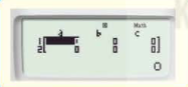
\includegraphics[width=0.8\linewidth]{imgs/9D1-2-casio-1.png}
        \item \hfill\par
        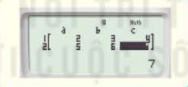
\includegraphics[width=0.8\linewidth]{imgs/9D1-2-casio-2.png}
        \item \hfill\par
        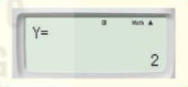
\includegraphics[width=0.8\linewidth]{imgs/9D1-2-casio-3.png}
    \end{cacbuoc}
\end{dhnh}

\tochucthuchien

\begin{tcth}
    \buocmot
    \item GV yêu cầu HS tự đọc thông tin từ phần Đọc hiểu - Nghe hiểu và thực hiện theo các bước.\\
    \textit{Lưu ý: GV hướng dẫn phù hợp với loại máy tính mà HS đang sử dụng. }
    \buochai
    \item HS đọc thông tin và thực hiện với MTCT của mình. 
    \item GV quan sát và hỗ trợ HS trong lúc thực hành. 
    \buocba
    \item HS thảo luận cách dùng MTCT.
    \buocbon
    \item GV đưa ra Chú ý:
    \begin{chuy}
        \begin{itemize}
            \item Muốn xoá số vừa mới nhập thì bấm phím \fbox{AC}; muốn thay đổi số đã nhập ở một vị trí nào đó thì di chuyển con trỏ đến vị trí đó rồi nhập số mới.
            \item Bấm phím \fbox{$\blacktriangle$} hay \fbox{$\blacktriangledown$} để chuyển đổi hiển thị các giá trị của $x$ và $y$ trong kết quả.
            \item Nếu máy báo ``Infinite Sol'' thì hệ phương trình đã cho có vô số nghiệm. Nếu máy báo ``No--Solution'' thì hệ phương trình đã cho vô nghiệm.
        \end{itemize}
    \end{chuy}
\end{tcth}

\paragraph{Hoạt động luyện tập}

\muctieu

\begin{itemize}
    \item Củng cố kĩ năng tìm nghiệm của hệ hai phương trình trình bậc nhất hai ẩn bằng MTCT.
\end{itemize}

\noidungsanpham

\begin{thuchanh}
    Dùng MTCT thích hợp để tìm nghiệm của các hệ phương trình sau:
    \begin{listEX}[2]
        \item $\heva{&2x + 3y = -4 \\ &-3x - 7y = 13;}$
        \item $\heva{&2x + 3y = 1 \\ &-x - 1,5y = 1;}$
        \item $\heva{&8x - 2y - 6 = 0 \\ &4x - y - 3 = 0.}$
    \end{listEX}
    %%%
    \doicot
    %%%
    \huongdan
    \begin{listEX}
        \item Hệ phương trình có nghiệm là $\left(\dfrac{11}{5};\dfrac{-11}{5}\right)$;
        \item Hệ phương trình vô nghiệm;
        \item Hệ phương trình có vô số nghiệm:
        $$(x;4x-3)\text{ với }x\in\mathbb{R}.$$
    \end{listEX}
\end{thuchanh}

\tochucthuchien

\begin{tcth}
    \buocmot
    \item GV tổ chức cho HS thực hành giải hệ phương trình bằng 
    \buochai
    \item HS thực hiện dưới sự hướng dẫn của GV. 
    \buocba
    \item HS giờ tay phát biểu.
    \buocbon
    \item GV nhận xét và giải đáp thắc mắc của HS. Chú ý hướng dẫn HS đưa ra dạng nghiệm tổng quát ở ý c.
\end{tcth}

\paragraph{Hoạt động vận dụng}

\muctieu

\begin{itemize}
    \item  Giúp học sinh vận dụng kiến thức về giải hệ hai phương trình bậc nhất hai ẩn để giải quyết một bài toán liên quan đến Hóa học.
\end{itemize}

\noidungsanpham

\begin{vandung}
    Thực hiện lần lượt các yêu cầu sau để tính số mililít dung dịch acid HCl nồng độ 20 \% và số mililít dung dịch acid HCl nồng độ 5 \% cần dùng để pha chế 2 lít dung dịch acid HCl nồng độ 10 \%.
    \begin{listEX}
        \item Gọi $x$ là số mililít dung dịch acid HCl nồng độ 20\%, $y$ là số mililít dung dịch acid HCl nồng độ 5\% cần lấy. Hãy biểu thị qua $x$ và $y$:
        \begin{itemize}
            \item Thể tích của dung dịch acid HCl 10\% nhận được sau khi trộn lẫn hai dung dịch acid ban đầu.
            \item Tổng số mililít acid HCl nguyên chất có trong hai dung dịch acid này.
        \end{itemize}
        \item Sử dụng kết quả ở câu a, hãy lập một hệ hai phương trình bậc nhất với hai ẩn là $x$, $y$. Giải hệ phương trình này để tính số mililít cần lấy của mỗi dung dịch acid HCl ở trên.
    \end{listEX}
    %%%
    \doicot
    %%%
    \huongdan\\
    Ta có hệ phương trình:
    $$\heva{&x+y=2000\\&\dfrac{0{,}2x+0{,}05y}{2000}}=0,1.$$
    Giải hệ phương trình trên, ta được:
    $$x=\dfrac{2000}{y};y=\dfrac{4000}{3}.$$
\end{vandung}

\begin{phieuhoctap}
	Xem Phiếu học tập 1 ở mục Phụ lục.
	%%%
	\doicot
	%%%
	\huongdan\\
	\textbf{Câu 1.} C\\
	\textbf{Câu 2.} C\\
	\textbf{Câu 3.} D\\
	\textbf{Câu 4.} A\\
	\textbf{Câu 5.} B\\
	\textbf{Câu 6.} D
\end{phieuhoctap}

\tochucthuchien

\begin{tcth}[vandung=3]
    \buocmot
    \item GV tổ chức cho HS làm việc nhóm đôi để thảo luận thực hiện nhiệm vụ của phần Vận dụng
    \buochai
    \item HS làm việc theo nhóm dưới sự hướng dẫn của GV. 
    \buocba
    \item GV gọi đại diện 2 nhóm lên bảng trình bày.
    \item Các nhóm khác nhận xét.
    \buocbon
    \item GV phân tích, nhận xét bài làm của HS.
\end{tcth}

\begin{tcth}[phieuhoctap=1]
	\buocmot
	\item HS làm theo nhóm bốn vào phiếu học tập số 1.
	\buochai
	\item HS làm việc theo nhóm dưới sự hướng dẫn của GV. 
	\buocba
	\item GV gọi đại diện các nhóm đưa ra đáp án từng câu.
	\item Các nhóm khác nhận xét.
	\buocbon
	\item GV phân tích, nhận xét câu trả lời của HS.
\end{tcth}

\subsubsection{Chữa bài tập cuối bài trong SGK}

\paragraph{Hoạt động khởi động}

\muctieu

\begin{itemize}
    \item HS nhớ lại các cách giải hệ hai phương trình bậc nhất hai ẩn đã học. 
\end{itemize}

\noidungsanpham

\begin{phieuhoctap}
	Xem Phiếu học tập 2 ở mục Phụ lục.
	%%%
	\doicot
	%%%
	\huongdan\\
	\textbf{Câu 1.} Biểu diễn, thế, một, một ẩn, nghiệm.\\
	\textbf{Câu 2.} Bằng nhau, đối nhau, cộng, trừ, một ẩn, một ẩn, nghiệm.
\end{phieuhoctap}

\tochucthuchien

\begin{tcth}
    \buocmot
    \item GV cho HS hoạt động theo cặp trong 3 phút để hoàn thành phiếu học tập số 2 trong Phụ lục.
    \buochai
    \item HS thực hiện phiếu học tập số 2. 
    \buocba
    \item HS giơ tay phát biểu.
    \item Các HS khác theo dõi bài làm, nhận xét và góp ý.
    \buocbon
    \item GV tổng kết.
\end{tcth}

\paragraph{Hoạt động luyện tập}

\muctieu

\begin{itemize}
    \item Củng cố cách giải hệ hai phương trình bậc nhất hai ẩn bằng phương pháp thế, phương pháp cộng đại số hoặc sử dụng máy tính cầm tay.
\end{itemize}

\noidungsanpham

\begin{baitap}[1.6]
    Giải các hệ phương trình sau bằng phương pháp thế:
    \begin{listEX}[2]
        \item $\heva{&x - y = 3 \\ &3x - 4y = 2;}$
        \item $\heva{&7x - 3y = 13 \\ &4x + y = 2;}$
        \item $\heva{&0,5x - 1,5y = 1 \\ &-x + 3y = 2.}$
    \end{listEX}
    %%%
    \doicot
    %%%
    \huongdan
    \begin{listEX}
    	\item $(10;7)$;
    	\item $(1;-2)$;
    	\item Vô nghiệm.
    \end{listEX}
\end{baitap}

\begin{baitap}[1.7]
    Giải các hệ phương trình sau bằng phương pháp cộng đại số:
    \begin{listEX}[2]
        \item $\heva{&3x + 2y = 6 \\ &2x - 2y = 14;}$
        \item $\heva{&0,3x + 0,5y = 3 \\ &1,5x - 2y = 1,5;}$ 
        \item $\heva{&-2x + 6y = 8 \\ &3x - 9y = -12.}$
    \end{listEX}
    %%%
    \doicot
    %%%
    \huongdan
    \begin{listEX}
    	\item $(4;-3)$;
    	\item $(5;3)$;
    	\item Vô số nghiệm: $\left(x;\dfrac{x+4}{3}\right)$ với $x\in\mathbb{R}$.
    \end{listEX}
\end{baitap}

\begin{baitap}[1.8]
    Cho hệ phương trình $\heva{&2x - y = -3 \\ &-2m^2x + 9y = 3(m + 3)}$, trong đó $m$ là số đã cho. Giải hệ phương trình trong mỗi trường hợp sau:
    \begin{listEX}[3]
        \item $m = -2$;
        \item $m = -3$;
        \item $m = 3$.
    \end{listEX}
    %%%
    \doicot
    %%%
    \huongdan
    \begin{listEX}
    	\item $\left(-\dfrac{12}{5};-\dfrac{9}{5}\right)$;
    	\item Vô nghiệm;
    	\item Vô nghiệm.
    \end{listEX}
\end{baitap}

\begin{baitap}[1.9]
    Dùng MTCT thích hợp để tìm nghiệm của các hệ phương trình sau:
    \begin{listEX}
        \item $\heva{&12x - 5y + 24 = 0 \\ &-5x - 3y - 10 = 0;}$
        \item $\heva{&\frac{1}{3}x - y = \frac{2}{3} \\ &x - 3y = 2;}$
        \item $\heva{&3x - 2y = 1 \\ &-x + \frac{2}{3}y = 0;}$
        \item $\heva{&\frac{4}{9}x - \frac{3}{5}y = 11 \\ &\frac{2}{9}x + \frac{1}{5}y = -2.}$
    \end{listEX}
    %%%
    \doicot
    %%%
    \huongdan
    \begin{listEX}
    	\item $(-2;0)$;
    	\item Vô số nghiệm: $\left(x;\dfrac{1}{2}x-\dfrac{2}{3}\right)$ với $x\in\mathbb{R}$;
    	\item Vô nghiệm;
    	\item $\left(\dfrac{9}{2};-15\right)$.
    \end{listEX}
\end{baitap}

\tochucthuchien

\begin{tcth}[baitap={từ 1.6 đến 1.9}]
	\buocmot
	\item GV tổ chức cho HS làm cá nhân.
	\buochai
	\item HS làm bài vào vở.
	\item GV mời HS làm bài.
	\buocba
	\item Các HS khác nhận xét bài làm của bạn.
	\buocbon
	\item GV nhận xét, chỉnh sửa nếu cần. 
\end{tcth}

\subsection{Phụ lục}

\paragraph{Phiếu học tập số 1}

\begin{ex}
Cho hệ phương trình $\heva{&x - y = 8 \\ &2x + 3y = -9}$. Cho các khẳng định sau:
\begin{itemize}
    \item[(i)] Từ phương trình thứ nhất của hệ, biểu diễn $y$ theo $x$ ta được: $y = x - 8$.
    \item[(ii)] Từ phương trình thứ nhất của hệ, biểu diễn $x$ theo $y$ ta được: $x = 8 - y$.
    \item[(iii)] Nghiệm của hệ là cặp số $(3; -5)$.
\end{itemize}
Số khẳng định đúng trong các khẳng định trên là
\choice
{0}
{1}
{2}
{3}
\end{ex}

\begin{ex}
Cho hệ phương trình $\heva{&\dfrac{1}{2}x - \dfrac{1}{2}y = -1 \\ &-3x + 3y = 5}$. Cho các khẳng định sau:
\begin{itemize}
    \item[(i)] Nhân phương trình thứ nhất của hệ với 6, rồi cộng với phương trình thứ hai ta được phương trình: $6y = -1$.
    \item[(ii)] Nhân phương trình thứ nhất của hệ với 6, rồi cộng với phương trình thứ hai ta được phương trình: $0x = -1$.
    \item[(iii)] Hệ phương trình đã cho vô nghiệm.
    \item[(iv)] Hệ phương trình đã cho có nghiệm.
\end{itemize}
Số khẳng định đúng trong các khẳng định trên là
\choice
{0}
{1}
{2}
{3}
\end{ex}

\begin{ex}
Biết rằng nghiệm của hệ phương trình $\heva{&2x + y = 4 \\ &6x - 5y = -12}$ là $(a; b)$. Giá trị của $T = 2a + 3b$ là
\choice
{8}
{-8}
{11}
{10}
\end{ex}

\begin{ex}
Biết rằng nghiệm của hệ phương trình $\heva{&-3x + y = 7 \\ &3x - 4y = -10}$ là $(a; b)$. Giá trị của $T = a^3 + b^3$ là
\choice
{-7}
{9}
{-9}
{7}
\end{ex}

\begin{ex}
Cho hệ phương trình $\heva{&2x - 3y = -1 \\ &-6x + 9y = 3}$. Khẳng định nào sau đây là SAI?
\choice
{Hệ đã cho có nghiệm là $\left(2; \dfrac{5}{3}\right)$}
{Hệ đã cho vô nghiệm}
{Hệ đã cho có nghiệm là $(4; 3)$}
{Hệ đã cho có nghiệm là $\left(x, \dfrac{2}{3}x + \dfrac{1}{3}\right)$ với $x \in \mathbb{R}$}
\end{ex}

\begin{ex}
Hệ phương trình nào sau đây vô nghiệm?
\choice
{$\heva{&x + 2y = 4 \\ &3x - y = -5}$}
{$\heva{&3x - 2y = 5 \\ &-12x + 8y = -20}$}
{$\heva{&5x + 2y = -1 \\ &4x - 3y = 6}$}
{$\heva{&-4x + 3y = -1 \\ &8x - 6y = -2}$}
\end{ex}

\paragraph{Phiếu học tập số 2}

\begin{bt}
    Điền vào chỗ trống cho phù hợp:
    \begin{center}
        \textbf{Cách giải hệ phương trình bằng phương pháp thế}
    \end{center}
    \begin{cacbuoc}
        \item Từ một phương trình của hệ, \makebox[3cm]{\dotfill} một ẩn theo ẩn kia rồi \makebox[3cm]{\dotfill} vào phương trình còn lại của hệ để được phương trình chỉ còn chứa \makebox[3cm]{\dotfill} ẩn.
        \item Giải phương trình \makebox[3cm]{\dotfill} vừa nhận được, từ đó suy ra \makebox[3cm]{\dotfill} của hệ đã cho.
    \end{cacbuoc}
\end{bt}

\begin{bt}
    Điền vào chỗ trống cho phù hợp:
    \begin{center}
        \textbf{Cách giải hệ phương trình bằng phương pháp cộng đại số}
    \end{center}
    Để giải một hệ hai phương trình bậc nhất hai ẩn có hệ số của cùng một ẩn nào đó trong hai phương trình \makebox[3cm]{\dotfill} hoặc \makebox[3cm]{\dotfill}, ta có thể làm như sau:
    \begin{cacbuoc}
        \item \makebox[3cm]{\dotfill} hay \makebox[3cm]{\dotfill} từng vế của hai phương trình trong hệ để được phương trình chỉ còn chứa \dots\dots\dots\dots\dots\dots .
        \item Giải phương trình \makebox[3cm]{\dotfill} vừa nhận được, từ đó suy ra \makebox[3cm]{\dotfill} của hệ đã cho.
    \end{cacbuoc}
\end{bt}

	\newpage
	\def\thoigian{2}
\section*
{Luyện tập chung}

\subsection{Mục tiêu}

\paragraph{Về kiến thức, kĩ năng}

\begin{itemize}
	\item Luyện tập giải hệ phương trình bậc nhất hai ẩn bằng phương pháp thế hay phương pháp cộng đại số.
	\item Luyện tập tìm nghiệm của hệ hai phương trình bậc nhất hai ẩn bằng máy tính cầm tay.
\end{itemize}

\paragraph{Về năng lực}

\begin{itemize}
	\item Rèn luyện năng lực toán học, nói riêng là năng lực tư duy và lập luận toán học, năng lực sử dụng công cụ, phương tiện học toán.
	\item Bồi dưỡng hứng thú học tập, ý thức làm việc nhóm, ý thức tìm tòi, khám phá và sáng tạo cho HS. 
\end{itemize}

\paragraph{Về phẩm chất}

\begin{itemize}
	\item Góp phần giúp HS rèn luyện và phát triển các phẩm chất tốt đẹp (yêu nước, nhân ái, chăm chỉ, trung thực, trách nhiệm):
	\begin{itemize}
		\item Tích cực phát biểu, xây dựng bài và tham gia các hoạt động nhóm;
		\item Có ý thức tích cực tìm tòi, sáng tạo trong học tập; phát huy điểm mạnh, khắc phục các điểm yếu của bản thân. 
	\end{itemize}
\end{itemize}

\subsection{Thiết bị dạy học và học liệu}

\paragraph{Giáo viên}

\begin{itemize}
	\item Giáo án, bảng phụ, máy chiếu (nếu có), phiếu học tập, … 
\end{itemize}

\paragraph{Học sinh}

\begin{itemize}
	\item SGK, vở ghi, dụng cụ học tập, máy tính cầm tay. 
\end{itemize}

\subsection{Tiến trình dạy học}

Bài học này dạy trong 02 tiết:

\begin{itemize}
	\item Tiết 1: Ôn lại lí thuyết và các ví dụ.
	\item Tiết 2: Các bài tập cuối bài.
\end{itemize}

\subsubsection{Ôn tập lý thuyết và các ví dụ}

\paragraph{Hoạt động khởi động}

\subparagraph{Mục tiêu}

\begin{itemize}
	\item Hệ thống lại kiến thức về các phương pháp giải hệ hai phương trình bậc nhất hai ẩn.
\end{itemize}

\begin{paracol}{2}
	\subparagraph{Nội dung}
	\switchcolumn
	\subparagraph{Sản phẩm}
\end{paracol}

\begin{ontap}
	Nhắc lại các bước để giải hệ hai phương trình bậc nhất hai ẩn bằng:
	\begin{listEX}
		\item phương pháp thế;
		\item phương pháp cộng đại số.
	\end{listEX}
	%%%
	\doicot
	%%%
	\begin{listEX}
		\item Giải hệ phương trình bằng phương pháp thế:
		\begin{itemize}
			\item \textit{Bước 1.} Từ một phương trình của hệ, biểu diễn một ẩn theo ẩn kia rồi thế vào phương trình còn lại của hệ để được phương trình chỉ còn chứa một ẩn.
			\item \textit{Bước 2.} Giải phương trình một ẩn vừa nhận được, từ đó suy ra nghiệm của hệ đã cho.
		\end{itemize}
		\item Giải hệ phương trình bằng phương pháp cộng đại số:
		\begin{itemize}
			\item \textit{Bước 1.} Cộng hay trừ từng vế của hai phương trình trong hệ để được phương trình chỉ còn chứa một ẩn.
			\item \textit{Bước 2.} Giải phương trình một ẩn vừa nhận được, từ đó suy ra nghiệm của hệ phương trình đã cho.
		\end{itemize}
	\end{listEX}
\end{ontap}

\subparagraph{Tổ chức thực hiện}

\begin{tcth}
	\buocmot
	\item GV cho HS nhắc lại các bước để giải hệ hai phương trình bậc nhất hai ẩn bằng phương pháp thế và phương pháp cộng đại số.
	\buochai
	\item HS suy nghĩ, chuẩn bị câu trả lời.
	\buocba
	\item HS giơ tay phát biểu.
	\item Các HS khác nhận xét.
	\buocbon
	\item GV nhận xét và nhắc lại các lưu ý khi sử dụng các phương pháp này.
\end{tcth}

\paragraph{Hoạt động luyện tập}

\subparagraph{Mục tiêu}

\begin{itemize}
	\item Củng cố kĩ năng giải hệ hai phương trình bậc nhất hai ẩn.
\end{itemize}

\begin{paracol}{2}
	\subparagraph{Nội dung}
	\switchcolumn
	\subparagraph{Sản phẩm}
\end{paracol}

\begin{vidu}
	Giải hệ phương trình $\heva{&0,5x + 0,6y = 0,4 \\ &0,4x - 0,9y = 1,7.}$
	%%%
	\doicot
	%%%
	Nhân hai vế của mỗi phương trình với 10, ta được:
	$$\heva{&5x + 6y = 4 \\ &4x - 9y = 17.} \quad (1)$$
	Ta giải hệ (1). Nhân hai vế của phương trình thứ nhất với 3 và nhân hai vế của phương trình thứ hai với 2, ta được hệ:
	$$\heva{&15x + 18y = 12 \\ &8x - 18y = 34.} \quad (2)$$
	Cộng từng vế hai phương trình của hệ (2) ta được $23x = 46$, suy ra $x = 2$.\\
	Thế $x = 2$ vào phương trình thứ nhất của hệ (1), ta được $5 \cdot 2 + 6y = 4$ hay $6y = -6$, suy ra $y = -1$.\\
	Vậy hệ phương trình đã cho có nghiệm là $(2; -1)$.
\end{vidu}

\begin{vidu}
	Tìm các hệ số $x, y$ trong phản ứng hoá học đã được cân bằng sau:
	$$\ce{3Fe + xO2 -> yFe3O4}.$$
	%%%
	\doicot
	%%%	
	Vì số nguyên tử của $\text{Fe}$ và $\text{O}$ ở cả hai vế của phương trình phản ứng phải bằng nhau nên ta có hệ phương trình $\heva{&3 = 3y \\ &2x = 4y}$ hay $\heva{&y = 1 \\ &x = 2y.}$\\
	Giải hệ này ta được $x = 2, y = 1$.
\end{vidu}

\begin{vidu}
	Tìm hai số $a$ và $b$ để đường thẳng $y = ax + b$ đi qua hai điểm $A(-2; -1)$ và $B(2; 3)$.
	%%%
	\doicot
	%%%
	Đường thẳng $y = ax + b$ đi qua điểm $A(-2; -1)$ nên $a(-2) + b = -1$ hay $-2a + b = -1$.\\
	Tương tự, đường thẳng $y = ax + b$ đi qua điểm $B(2; 3)$ nên $a \cdot 2 + b = 3$ hay $2a + b = 3$.\\
	Từ đó, ta có hệ phương trình với hai ẩn là $a$ và $b$:
	$$\heva{&-2a + b = -1 \\ &2a + b = 3.}$$
	Cộng từng vế hai phương trình của hệ, ta được $2b = 2$, suy ra $b = 1$.\\
	Thay $b = 1$ vào phương trình thứ nhất, ta có $-2a + 1 = -1$, suy ra $a = 1$.\\
	Vậy với $a = 1, b = 1$ thì đường thẳng $y = ax + b$ đi qua hai điểm $A, B$ đã cho.
\end{vidu}

\subparagraph{Tổ chức thực hiện}

\noindent\faBookmarkO~\textit{\textbf{Ví dụ 1:}}

\begin{tcth}
	\buocmot
	\item GV yêu cầu HS làm việc cá nhân.
	\buochai
	\item HS thực hiện theo hướng dẫn của GV.
	\buocba
	\item Sau đó, GV gọi HS	lên bảng trình bày lời giải.
	\item Các HS khác nhận xét.
	\buocbon
	\item Sau đó GV tổng kết và lưu ý sai lầm thường mắc cho HS.
\end{tcth}

\noindent\faBookmarkO~\textit{\textbf{Ví dụ 2:}}

\begin{tcth}
	\buocmot
	\item GV tổ chức để HS nhớ lại các kiến thức Hóa học về cân bằng phương trình.
	\item GV yêu cầu HS làm việc nhóm đôi.
	\buochai
	\item HS thực hiện theo hướng dẫn của GV.
	\buocba
	\item Sau đó, GV gọi HS	lên bảng trình bày lời giải.
	\item Các HS khác nhận xét.
	\buocbon
	\item Sau đó GV tổng kết và lưu ý sai lầm thường mắc cho HS.
\end{tcth}

\noindent\faBookmarkO~\textit{\textbf{Ví dụ 3:}}

\begin{tcth}
	\buocmot
	\item GV tổ chức để HS nhớ lại các kiến thức Hình học về đồ thị hàm số bậc nhất, GV cần yêu cầu HS nhắc lại	về điều kiện để một điểm cho trước thuộc đồ thị hàm số bậc nhất.
	\item GV yêu cầu HS làm việc cá nhân.
	\buochai
	\item HS thực hiện theo hướng dẫn của GV.
	\buocba
	\item Sau đó, GV gọi HS	lên bảng trình bày lời giải.
	\item Các HS khác nhận xét.
	\buocbon
	\item Sau đó GV tổng kết và lưu ý sai lầm thường mắc cho HS.
\end{tcth}

\paragraph{Tổng kết và hướng dẫn công việc về nhà}

GV tổng kết lại nội dung bài học và dặn dò công việc ở nhà cho HS:

\begin{itemize}
	\item GV tổng kết lại các kiến thức trọng tâm của bài học: Các cách giải hệ hai phương trình bậc nhất hai ẩn.
	\item Nhắc HS về nhà ôn tập các nội dung đã học.
\end{itemize}

\subsubsection{Các bài tập cuối bài}

\paragraph{Hoạt động luyện tập}

\subparagraph{Mục tiêu}

\begin{itemize}
	\item Củng cố giải hệ phương trình bậc nhất hai ẩn bằng phương pháp thế, phương pháp cộng đại số hoặc sử dụng máy tính cầm tay.
\end{itemize}

\begin{paracol}{2}
	\subparagraph{Nội dung}
	\switchcolumn
	\subparagraph{Sản phẩm}
\end{paracol}

\begin{baitap}[1.10]
	Cho hai phương trình:
	\begin{align*}
		-2x + 5y &= 7; \quad (1) \\
		4x - 3y &= 7. \quad (2)
	\end{align*}
	Trong các cặp số $(2; 0)$, $(1; -1)$, $(-1; 1)$, $(-1; 6)$, $(4; 3)$ và $(-2; -5)$, cặp số nào là:
	\begin{listEX}
		\item Nghiệm của phương trình (1)?
		\item Nghiệm của phương trình (2)?
		\item Nghiệm của hệ gồm phương trình (1) và \\
		phương trình (2)?
	\end{listEX}
	%%%
	\doicot
	%%%
	\huongdan
	\begin{listEX}
		\item Nghiệm của phương trình (1): $(-1 ; 1)$, $(4 ; 3)$.
		\item Nghiệm của phương trình (2): $(1 ; -1)$, $(4 ; 3)$, $(- 2; -5)$.
		\item Nghiệm của hệ gồm (1) và (2): $(4 ; 3)$.
	\end{listEX}
\end{baitap}

\begin{baitap}[1.11]
	Giải các hệ phương trình sau bằng phương pháp thế:
	\begin{listEX}
		\item $\heva{&2x - y = 1 \\ &x - 2y = -1;}$
		\item $\heva{&0,5x - 0,5y = 0,5 \\ &1,2x - 1,2y = 1,2;}$
		\item $\heva{&x + 3y = -2 \\ &5x - 4y = 28.}$
	\end{listEX}
	%%%
	\doicot
	%%%
	\huongdan
	\begin{listEX}
		\item $(1;1)$;
		\item Vô số nghiệm: $(x;x-1)$ với $x\in\mathbb{R}$;
		\item $(4;-2)$.
	\end{listEX}
\end{baitap}

\begin{baitap}[1.12]
	Giải các hệ phương trình sau bằng phương pháp cộng đại số:
	\begin{listEX}
		\item $\heva{&5x + 7y = -1 \\ &3x + 2y = -5;}$
		\item $\heva{&2x - 3y = 11 \\ &-0,8x + 1,2y = 1;}$
		\item $\heva{&4x - 3y = 6 \\ &0,4x + 0,2y = 0,8.}$
	\end{listEX}
	%%%
	\doicot
	%%%
	\huongdan
	\begin{listEX}
		\item $(-3;2)$;
		\item Vô nghiệm;
		\item $(1{,}8;0{,}4)$.
	\end{listEX}
\end{baitap}

\begin{baitap}[1.13]
	Tìm các hệ số $x$, $y$ trong phản ứng hoá học đã được cân bằng sau:
	$$\ce{4Al + xO2 -> yAl2O3}.$$
	%%%
	\doicot
	%%%
	\huongdan\\
	$x=3$, $y=2$.
\end{baitap}

\begin{baitap}[1.14]
	Tìm $a$ và $b$ sao cho hệ phương trình 
	$$\heva{&ax + by = 1 \\ &ax + (2 - b)y = 3}$$ 
	có nghiệm là $(1; -2)$.
	%%%
	\doicot
	%%%
	\huongdan\\
	Vì $(x; y) = (1; -2)$ là nghiệm của hệ đã cho nên ta có:
	$$\heva{&a - 2b = 1 \\ &a + 2(b - 2) = 3} \quad \text{hay} \quad \heva{&a - 2b = 1 \\ &a + 2b = 7.}$$
	Giải hệ này ta được $a = 4, b = \dfrac{3}{2}$.
\end{baitap}

\subparagraph{Tổ chức thực hiện}

\textit{(Dùng chung cho các bài tập từ 1.10 đến 1.14)}

\begin{tcth}
	\buocmot
	\item GV tổ chức cho HS làm cá nhân.
	\buochai
	\item HS làm bài vào vở
	\item GV mời HS lên bảng làm bài.
	\buocba
	\item Các HS khác nhận xét bài làm của bạn.
	\buocbon
	\item GV nhận xét, chỉnh sửa nếu cần. 
	\item HS sửa bài.
\end{tcth}

\paragraph{Tổng kết và hướng dẫn cộng việc ở nhà}

GV tổng kết lại nội dung bài học và dặn dò công việc ở nhà cho HS:

\begin{itemize}
	\item GV tổng kết lại các kiến thức trọng tâm của bài học: Tóm tắt cách giải hệ hai phương trình bậc nhất hai ẩn bằng phương pháp thế, phương pháp cộng đại số, dùng máy tính cầm tay.
\end{itemize}
	\newpage
	\def\thoigian{2}
\section
[Giải bài toán bằng cách lập hệ phương trình]
{GIẢI BÀI TOÁN BẰNG CÁCH LẬP HỆ PHƯƠNG TRÌNH}

\subsection{MỤC TIÊU}

\paragraph{Về kiến thức, kĩ năng}

\begin{itemize}
	\item Giải một số bài toán bằng cách lập hệ hai phương trình bậc nhất hai ẩn.
\end{itemize}

\paragraph{Về năng lực}

\begin{itemize}
	\item Rèn luyện năng lực toán học, nói riêng là năng lực mô hình hoá toán học và năng lực giải quyết vấn đề toán học.
	\item Bồi dưỡng hứng thú học tập, ý thức làm việc nhóm, ý thức tìm tòi, khám phá và sáng tạo cho HS. 
\end{itemize}

\paragraph{Về phẩm chất}

\begin{itemize}
	\item Góp phần giúp HS rèn luyện và phát triển các phẩm chất tốt đẹp (yêu nước, nhân ái, chăm chỉ, trung thực, trách nhiệm):
	\begin{itemize}
		\item Tích cực phát biểu, xây dựng bài và tham gia các hoạt động nhóm;
		\item Có ý thức tích cực tìm tòi, sáng tạo trong học tập; phát huy điểm mạnh, khắc phục các điểm yếu của bản thân. 
	\end{itemize}
\end{itemize}

\subsection{THIẾT BỊ DẠY HỌC VÀ HỌC LIỆU}

\paragraph{Giáo viên}

\begin{itemize}
	\item Giáo án, bảng phụ, máy chiếu (nếu có),… 
\end{itemize}

\paragraph{Học sinh}

\begin{itemize}
	\item SGK, vở ghi, dụng cụ học tập.
\end{itemize}

\subsection{TIẾN TRÌNH DẠY HỌC}

\danhsachtiet

\subsubsection{Giải bài toán bằng cách lập hệ phương trình}

\paragraph{Hoạt động khởi động}

\muctieu

\begin{itemize}
	\item Gợi động cơ, tạo tình huống xuất hiện trong thực tế để HS vận dụng kiến thức về giải hệ phương trình để giải quyết tính huống.
\end{itemize}

\noidungsanpham

\begin{modau}
	Một vật có khối lượng $124$ g và thể tích $15$ cm$^3$ là hợp kim của đồng và kẽm. TÍnh xem trong đó có bao nhiêu gam đồng và bao nhiêu gam kẽm, biết rằng $1$ cm$^3$ đồng nặng $8{,}9$ g và $1$ cm$^3$ kẽm nặng $7$ g.
\end{modau}

\tochucthuchien

\begin{tcth}
	\buocmot
	\item GV yêu cầu HS đọc tình huống thực tế và cho biết có bao nhiêu đại lượng chưa biết trong bài \textit{(GV giải thích lại thế nào là đại lượng nếu cần)}.
	\buochai
	\item HS suy nghĩ về tình huống mở đầu và nảy sinh nhu cầu tìm hiểu cách giải quyết tình hướng này.
	\buocba
	\item HS trả lời câu hỏi (không yêu cầu trả lời chính xác).
	\buocbon
	\item GV giới thiệu bài học mới về giải bài toán bằn cách lập hệ phương trình.
\end{tcth}

\paragraph{Hoạt động hình thành kiến thức}

\muctieu

\begin{itemize}
	\item HS nhận biết các bước thực hiện khi giải bài toán bằng cách lập hệ phương trình.
\end{itemize}

\noidungsanpham

\begin{ttkp}
	\textbf{Giải bài toàn bằng cách lập hệ phương trình}\\
	Xét bài toán ở Tình huống mở đầu. Gọi $x$ là số gam đồng, $y$ là số gam kẽm cần tính.
	\begin{itemize}
		\item[] \textbf{HĐ1:} Biểu thị khối lượng của vật qua $x$ và $y$.
		\item[] \textbf{HĐ2:} Biểu thị thể tích của vật qua $x$ và $y$.
		\item[] \textbf{HĐ3:} Giải hệ gồm hai phương trình bậc nhất hai ẩn $x$, $y$ nhận được ở \textbf{HĐ1} và \textbf{HĐ2}. Từ đó trả lời câu hỏi ở Tình huống mở đầu.
	\end{itemize}
	%%%
	\doicot
	%%%
	\huongdan
	\begin{itemize}
		\item[] \textbf{HĐ1:} Khối lượng của vật là $x+y$ (g).\\
		Mà khối lượng của vật đồng thời là $124$ g, nên 
		$$x+y=124\qquad(1)$$
		\item[] \textbf{HĐ2:} Thể tích của vật qua $\dfrac{x}{8{,}9}+\dfrac{y}{7}$ (cm$^3$).\\
		Mà thể tích của vật đồng thời là $15$ cm$^3$, nên 
		$$\dfrac{x}{8{,}9}+\dfrac{y}{7}=15\qquad(2)$$
		\item[] \textbf{HĐ3:} Từ (1) và (2), ta lập được hệ phương trình
		$$\heva{&x+y=124\\&\dfrac{x}{8{,}9}+\dfrac{y}{7}=15.}$$
		Giải hệ phương trình trên ta được:
		$$x=89;y=35$$
	\end{itemize}
\end{ttkp}

\begin{vidu}
	Tìm hai số tự nhiên có tổng bằng $1006$, biết rằng nếu lấy số lớn chia cho số nhỏ thì được thương là $2$ và số dư là $124$.
	%%%
	\doicot
	%%%
	\begin{itemize}
		\item Gọi hai số cần tìm là $x$ và $y$, trong đó $x < y$. Số dư trong phép chia $y$ cho $x$ là $124$ nên $x > 124$. Vậy điều kiện của hai ẩn là $x, y \in \mathbb{N}$ và $124 < x < y$.\\
		Tổng hai số bằng $1\,006$ nên ta có phương trình $x + y = 1\,006$.\\
		Khi chia $y$ cho $x$ ta được thương là $2$, dư $124$ nên ta có phương trình $y = 2x + 124$.\\
		Do đó, ta có hệ phương trình 
		$$\heva{&x + y = 1\,006 & (1) \\& y = 2x + 124. & (2) }$$
		\item Giải hệ phương trình: \\
		Từ (2) thế $y = 2x + 124$ vào (1), ta được $3x + 124 = 1\,006$ hay $3x = 882$, suy ra $x = 294$. \\
		Từ đó ta được $y = 2 \cdot 294 + 124 = 712$.
		\item Các giá trị $x = 294$ và $y = 712$ thoả mãn các điều kiện của ẩn. \\
		Vậy hai số cần tìm là $294$ và $712$.
	\end{itemize}
\end{vidu}

\tochucthuchien

\begin{tcth}[ttkp]
	\buocmot
	\item GV cho HS hoạt động cá nhân trong 5 phút. Sau đó, GV gọi một HS lên bảng trả lời hai HĐ1, 2; các HS khác quan sát, nhận xét và góp ý phần lời giải của HS. Tiếp theo GV gọi một HS khác lên làm HĐ3. 
	\buochai
	\item HS thực hiện theo hướng dẫn của GV.
	\buocba
	\item GV tổng kết suy ra cách giải bài toán bằng cách lập hệ phương trình.
	\buocbon
	\item GV viết bảng hoặc trình chiếu Nhận xét:
	\begin{nhanxet}
		Các bước giải một bài toán bằng cách lập hệ phương trình:
		\begin{cacbuoc}
			\item Lập hệ phương trình:
			\begin{itemize}
				\item Chọn ẩn số (thường chọn hai ẩn số) và đặt điều kiện thích hợp cho các ẩn số;
				\item Biểu diễn các đại lượng chưa biết theo ẩn và các đại lượng đã biết;
				\item Lập hệ phương trình biểu thị mối quan hệ giữa các đại lượng.
			\end{itemize}
			\item Giải hệ phương trình.
			\item Trả lời: Kiểm tra xem trong các nghiệm tìm được của hệ phương trình, nghiệm nào thoả mãn, nghiệm nào không thoả mãn điều kiện của ẩn, rồi kết luận.
		\end{cacbuoc}
	\end{nhanxet}
\end{tcth}

\begin{tcth}[vidu=1]
	\buocmot
	\item GV hướng dẫn HS lần lượt thực hiện theo ba Bước 1, 2, 3 nêu trong Nhận xét ở trên.
	\buochai
	\item HS làm bài vào vở dưới sự hướng dẫn của GV.
	\item GV gọi HS lên bảng làm bài.
	\buocba
	\item Các HS khác nhận xét. 
	\buocbon
	\item GV nhận xét, chỉnh sửa nếu cần.
\end{tcth}

\paragraph{Hoạt động luyện tập}

\muctieu

\begin{itemize}
	\item Củng cố kĩ năng giải bài toán bằng cách lập hệ phương trình.
\end{itemize}

\noidungsanpham

\begin{luyentap}
	Một chiếc xe khách đi từ Thành phố Hồ Chí Minh đến Cần Thơ, quãng đường dài $170\text{ km}$. Sau khi xe khách xuất phát $1$ giờ $40$ phút, một chiếc xe tải bắt đầu đi từ Cần Thơ về Thành phố Hồ Chí Minh (trên cùng một tuyến đường với xe khách) và gặp xe khách sau đó $40$ phút. Tính vận tốc của mỗi xe, biết rằng mỗi giờ xe khách đi nhanh hơn xe tải $15\text{ km}$.
	%%%
	\doicot
	%%%
	\huongdan\\
	Gọi $x\text{ (km/h)}$ là vận tốc của xe tải và $y\text{ (km/h)}$ là vận tốc xe khách ($x, y > 0$). Chú ý rằng hai xe (đi ngược chiều) gặp nhau khi tổng quãng đường hai xe đã đi bằng $170\text{ km}$.
\end{luyentap}

\begin{vidu}
	Hai đội công nhân cùng làm một đoạn đường trong $24$ ngày thì xong. Mỗi ngày, đội I làm được nhiều gấp rưỡi đội II. Hỏi nếu làm một mình thì mỗi đội làm xong đoạn đường đó trong bao lâu? (Giả sử năng suất của mỗi đội là không đổi).
	%%%
	\doicot
	%%%
	\begin{itemize}
		\item Gọi $x$ là số ngày để đội I hoàn thành công việc nếu làm một mình; $y$ là số ngày để đội II hoàn thành công việc nếu làm một mình. Điều kiện: $x > 0$ và $y > 0$.\\
		Mỗi ngày đội I làm được $\dfrac{1}{x}$ (công việc) và đội II làm được $\dfrac{1}{y}$ (công việc).\\
		Mỗi ngày đội I làm được nhiều gấp rưỡi đội II nên ta có phương trình $\dfrac{1}{x} = 1,5 \cdot \dfrac{1}{y}$ hay 
		$$\dfrac{1}{x} = \dfrac{3}{2} \cdot \dfrac{1}{y} \quad (1)$$
		Hai đội làm chung trong $24$ ngày thì xong công việc nên mỗi ngày, hai đội làm chung thì được $\dfrac{1}{24}$ (công việc). Ta có phương trình
		$$\dfrac{1}{x} + \dfrac{1}{y} = \dfrac{1}{24} \quad (2)$$
		Từ (1) và (2), ta có hệ phương trình 
		$$(I)\quad\heva{&\dfrac{1}{x} = \dfrac{3}{2} \cdot \dfrac{1}{y} \\ &\dfrac{1}{x} + \dfrac{1}{y} = \dfrac{1}{24}.}$$
		\item Nếu đặt $u = \dfrac{1}{x}$ và $v = \dfrac{1}{y}$ thì ta có hệ phương trình bậc nhất hai ẩn mới là $u$ và $v$:
		$$(II)\quad\heva{&u = \dfrac{3}{2}v & (3) \\ &u + v = \dfrac{1}{24}. & (4)}$$
		Giải hệ (II): Thế $u = \dfrac{3}{2}v$ vào phương trình (4), ta được $\dfrac{3}{2}v + v = \dfrac{1}{24}$, hay $\dfrac{5}{2}v = \dfrac{1}{24}$, suy ra $v = \dfrac{1}{60}$. Do đó $u = \dfrac{3}{2}v = \dfrac{3}{2} \cdot \dfrac{1}{60} = \dfrac{1}{40}$.\\
		Từ đó, ta có:
		$u = \dfrac{1}{x} = \dfrac{1}{40}$ suy ra $x = 40$; $v = \dfrac{1}{y} = \dfrac{1}{60}$ suy ra $y = 60$.
		\item Các giá trị tìm được của $x$ và $y$ thoả mãn điều kiện của ẩn.
	\end{itemize}
	\textit{Trả lời:} Nếu làm một mình thì đội I làm xong đoạn đường đó trong $40$ ngày, còn đội II làm xong trong $60$ ngày.
\end{vidu}

\begin{luyentap}
	Nếu hai vòi nước cùng chảy vào một bể không có nước thì bể sẽ đầy trong 1 giờ 20 phút. Nếu mở riêng vòi thứ nhất trong 10 phút và vòi thứ hai trong 12 phút thì chỉ được $\dfrac{2}{15}$ bể nước. Hỏi nếu mở riêng từng vòi thì thời gian để mỗi vòi chảy đầy bể nước là bao nhiêu phút?
	%%%
	\doicot
	%%%
	\huongdan\\
	Gọi $x$ (phút là thời gian vòi thứ nhất chảy đầy bể; $y$ (phút) là thời gian vòi thứ hai chảy đầy bể.\\
	Hệ phương trình:
	$$\heva{&80\left(\dfrac{1}{x}+\dfrac{1}{y}\right)=1\\&\dfrac{10}{x}+\dfrac{12}{y}=\dfrac{2}{15}.}$$
	Vòi thứ nhất: 120 phút, vòi thứ hai: 240 phút.
\end{luyentap}

\tochucthuchien

\begin{tcth}[luyentap=1]
	\buocmot
	\item GV cho HS hoạt động cá nhân.
	\buochai
	\item HS làm việc dưới sự hướng dẫn của GV.
	\item GV gọi HS lên bảng làm bài.
	\buocba
	\item Các HS khác nhận xét. 
	\buocbon
	\item GV nhận xét, chỉnh sửa nếu cần.
\end{tcth}

\begin{tcth}[vidu=2]
	\buocmot
	\item GV cần giải thích tương quan sau cho HS: ``Nếu đơn vị $A$ làm xong công việc (coi là $1$ công việc) trong $n$ ngày, thì mỗi ngày đơn vị $A$ làm $\dfrac{1}{n}$ công việc''.
	\item GV cho HS hoạt động cá nhân.
	\buochai
	\item HS làm việc dưới sự hướng dẫn của GV.
	\item GV gọi HS lên bảng làm bài.
	\buocba
	\item Các HS khác nhận xét. 
	\buocbon
	\item GV nhận xét, chỉnh sửa nếu cần.
	\item Lưu ý cho GV:\\
	\textit{Phương pháp đặt ẩn phụ không được trình bày tường minh trong SGK về mặt lí thuyết, GV cần lưu ý cho HS là tuy hệ (I) không phải là hệ bậc nhất hai ẩn, nhưng nếu ta đặt (ẩn phụ) $u=\dfrac{1}{x}$, $v=\dfrac{1}{y}$ thì ta lại được một hệ bậc nhất hai ẩn (II) đối với hai ẩn mới là $u$, $v$. Hệ này đơn giản hơn hệ (I) và HS đã biết cách giải.}
\end{tcth}

\begin{tcth}[luyentap=2]
	\buocmot
	\item GV cho HS hoạt động theo nhóm đôi.
	\buochai
	\item HS trao đổi nhóm để hoàn thành yêu cầu của Luyện tập 2.
	\item GV gọi 1 HS lên bảng làm bài.
	\buocba
	\item Các HS khác nhận xét. 
	\buocbon
	\item GV nhận xét, chỉnh sửa nếu cần.
\end{tcth}

\paragraph{Tổng kết và hướng dẫn công việc ở nhà}

GV tổng kết lại nội dung bài học và dặn dò công việc ở nhà cho HS:

\begin{itemize}
	\item GV tổng kết lại các kiến thức trọng tâm của bài học: Giải bài toán bằng cách lập hệ phương trình.
	\item Nhắc HS về nhà ôn tập các nội dung đã học.
	\item Giao cho HS làm các bài tập sau trong SGK: Bài 1.15 đến Bài 1.18.
\end{itemize}

\subsubsection{Chữa bài tập}

\paragraph{Hoạt động khởi động}

\muctieu

\begin{itemize}
	\item HS nhớ lại các cách giải bài toán bằng cách lập hệ phương trình bậc nhất hai ẩn.
\end{itemize}

\noidungsanpham

\begin{ontap}
	Nhắc lại các bước thực hiện khi giải bài toán bằng cách lập hệ phương trình.
	%%%
	\doicot
	%%%
	Các bước giải một bài toán bằng cách lập hệ phương trình:
	\begin{cacbuoc}
		\item Lập hệ phương trình:
		\begin{itemize}
			\item Chọn ẩn số (thường chọn hai ẩn số) và đặt điều kiện thích hợp cho các ẩn số;
			\item Biểu diễn các đại lượng chưa biết theo ẩn và các đại lượng đã biết;
			\item Lập hệ phương trình biểu thị mối quan hệ giữa các đại lượng.
		\end{itemize}
		\item Giải hệ phương trình.
		\item Trả lời: Kiểm tra xem trong các nghiệm tìm được của hệ phương trình, nghiệm nào thoả mãn, nghiệm nào không thoả mãn điều kiện của ẩn, rồi kết luận.
	\end{cacbuoc}
\end{ontap}

\tochucthuchien

\begin{tcth}
	\buocmot
	\item GV yêu cầu nhắc lại các bước thực	hiện khi giải bài toán bằng cách lập hệ	phương trình.
	\buochai
	\item HS chuẩn bị câu trả lời
	\buocba
	\item HS giơ tay phát biểu.
	\item Các HS khác nhận xét.
	\buocbon
	\item GV trình chiếu lại nội dung kiến thức và nhắc lại các bước cho HS.
\end{tcth}

\paragraph{Hoạt động luyện tập}

\muctieu

\begin{itemize}
	\item Củng cố kĩ năng giải bài toán bằng cách lập hệ phương trình.
\end{itemize}

\noidungsanpham

\begin{baitap}[1.15]
	Tìm số tự nhiên $n$ có hai chữ số, biết rằng tổng của hai chữ số đó bằng $12$, và nếu viết hai chữ số đó theo thứ tự ngược lại thì được một số lớn hơn $n$ là $36$ đơn vị.
	%%%
	\doicot
	%%%
	\huongdan\\
	Gọi $x$ là chữ số hàng chục, $y$ là chữ số hàng trăm (khi đó $n = 10x + y$). Điều kiện của ẩn là: $x, y \in \mathbb{N}$ và $0 < x \le 9$ và $0 \le y \le 9$. Ta có phương trình thứ nhất là $x + y = 12$. Khi viết hai chữ số của $n$ theo thứ tự ngược lại, ta được số $10y + x$.\\	
	Theo giả thiết ta có phương trình 
	$$(10y + x) - (10x + y) = 36,$$ 
	hay $9y - 9x = 36$.\\
	Từ đó ta có hệ phương trình
	$$\heva{&x+y=12\\&9y-9x=36.}$$
\end{baitap}

\begin{baitap}[1.16]
	Điểm số trung bình của một vận động viên bắn súng sau $100$ lần bắn là $8,69$ điểm. Kết quả cụ thể được ghi trong bảng sau, trong đó có hai ô bị mờ không đọc được (đánh dấu "?"):
	\begin{center}
		\begin{tblr}{|C{3cm}|c|c|c|c|c|}
			\hline
			Điểm số của mỗi lần bắn & 10 & 9 & 8 & 7 & 6 \\ \hline
			Số lần bắn & 25 & 42 & ? & 15 & ? \\ \hline
		\end{tblr}
	\end{center}
	Em hãy tìm lại các số bị mờ trong hai ô đó.
	%%%
	\doicot
	%%%
	\huongdan\\
	Gọi $x$ là số lần bắn được 8 điểm và $y$ là số lần bắn được 6 điểm. Điều kiện là $x, y \in \mathbb{N}$ (cũng có thể nêu điều kiện $x, y < 100$). Theo giả thiết, ta có hệ phương trình
	$$\heva{&25 + 42 + x + 15 + y = 100 \\ &(10 \cdot 25 + 9 \cdot 42 + 8x + 7 \cdot 15 + 6y) : 100 = 8{,}69}$$
	hay
	$$\heva{&x + y = 18 \\ &8x + 6y = 136.}$$
\end{baitap}

\begin{baitap}[1.17]
	Năm ngoái, hai đơn vị sản xuất nông nghiệp thu hoạch được $3\,600$ tấn thóc. Năm nay, hai đơn vị thu hoạch được $4\,095$ tấn thóc. Hỏi năm nay, mỗi đơn vị thu hoạch được bao nhiêu tấn thóc, biết rằng năm nay, đơn vị thứ nhất làm vượt mức $15\%$, đơn vị thứ hai làm vượt mức $12\%$ so với năm ngoái?\\	
	Hãy dùng máy tính cầm tay để kiểm tra lại kết quả thu được.
	%%%
	\doicot
	%%%
	\huongdan\\
	Gọi $x$ và $y$ lần lượt là số tấn thóc mà đơn vị thứ nhất và thứ hai thu hoạch được trong năm ngoái ($x, y > 0$). Ta có hệ phương trình
	$$\heva{&x + y = 3600 \\ &115\%x + 112\%y = 4095}$$
	hay
	$$\heva{&x + y = 3600 \\ &1,15x + 1,12y = 4095.}$$
\end{baitap}

\begin{baitap}[1.18]
	Hai người thợ cùng làm một công việc trong $16$ giờ thì xong. Nếu người thứ nhất làm trong $3$ giờ và người thứ hai làm trong $6$ giờ thì chỉ hoàn thành được $25\%$ công việc. Hỏi nếu làm riêng thì mỗi người hoàn thành công việc trong bao lâu?
	%%%
	\doicot
	%%%
	Gọi $x$ (giờ) là thời gian để người thứ nhất hoàn thành công việc, $y$ (giờ) là thời gian để người thứ hai hoàn thành công việc (điều kiện: $x > 0, y > 0$).\\
	Khi đó người thứ nhất mỗi giờ hoàn thành được $\dfrac{1}{x}$ công việc; người thứ hai được $\dfrac{1}{y}$ công việc.\\
	Cả hai cùng làm thì mỗi giờ được $\dfrac{1}{x} + \dfrac{1}{y}$ công việc, và hoàn thành toàn bộ công việc trong $16$ giờ nên ta có phương trình $16 \left( \dfrac{1}{x} + \dfrac{1}{y} \right) = 1$.\\
	Người thứ nhất làm trong $3$ giờ được $\dfrac{3}{x}$ công việc; người thứ hai làm trong $6$ giờ được $\dfrac{6}{y}$ công việc và khi đó cả hai chỉ hoàn thành được $25\%$ ($= \dfrac{1}{4}$) công việc nên ta có phương trình $\dfrac{3}{x} + \dfrac{6}{y} = \dfrac{1}{4}$.\\
	Ta có hệ phương trình (I) $\heva{&16 \left( \dfrac{1}{x} + \dfrac{1}{y} \right) = 1 \\ &\dfrac{3}{x} + \dfrac{6}{y} = \dfrac{1}{4}.}$\\
	Bằng cách đặt $u = \dfrac{1}{x}$ và $v = \dfrac{1}{y}$, ta đưa $(I)$ về dạng: (II) $\heva{&16(u + v) = 1 & (1) \\ &3u + 6v = \dfrac{1}{4} & (2)}$\\
	Giải hệ phương trình trên, ta được: Nếu làm riêng thì người thứ nhất hoàn thành công việc trong $24$ giờ, người thứ hai trong $48$ giờ.
\end{baitap}

\tochucthuchien

\begin{tcth}[baitap={từ 1.15 đến 1.18}]
	\buocmot
	\item GV cho HS làm bài cá nhân.
	\buochai
	\item HS làm bài vào vở.
	\item GV gọi 1 HS lên bảng làm bài.
	\buocba
	\item Các HS khác nhận xét. 
	\buocbon
	\item GV nhận xét, chỉnh sửa nếu cần.
\end{tcth}








	\newpage
	\def\thoigian{2}
\section
[Bài tập cuối chương I]
{BÀI TẬP CUỐI CHƯƠNG I}

\subsection{Mục tiêu}

\paragraph{Về kiến thức, kĩ năng}

\begin{itemize}
	\item Hệ thống các kiến thức đã học trong chương và cung cấp một số bài tập có nội dung tổng hợp, liên kết các kiến thức, kĩ năng đã học trong chương.
\end{itemize}

\paragraph{Về năng lực}

\begin{itemize}
	\item Rèn luyện năng lực toán học, nói riêng là năng lực mô hình hoá toán học, năng lực tư duy và lập luận toán học.
	\item Bồi dưỡng hứng thú học tập, ý thức làm việc nhóm, ý thức tìm tòi, khám phá và sáng tạo cho HS. 
\end{itemize}

\paragraph{Về phẩm chất}

\begin{itemize}
	\item Góp phần giúp HS rèn luyện và phát triển các phẩm chất tốt đẹp (yêu nước, nhân ái, chăm chỉ, trung thực, trách nhiệm): 
	\begin{itemize}
		\item Tích cực phát biểu, xây dựng bài và tham gia các hoạt động nhóm; 
		\item Có ý thức tích cực tìm tòi, sáng tạo trong học tập; phát huy điểm mạnh, khắc phục các điểm yếu của bản thân. 
	\end{itemize}
\end{itemize}

\subsection{Thiết bị dạy học và học liệu}

\paragraph{Giáo viên}

\begin{itemize}
	\item Giáo án, bảng phụ, máy chiếu (nếu có), giấy A3, … 
\end{itemize}

\paragraph{Học sinh}

\begin{itemize}
	\item SGK, vở ghi, dụng cụ học tập, máy tính cầm tay.
\end{itemize}

\subsection{Tiến trình dạy học}

\danhsachtiet

\subsubsection
[Ôn tập lí thuyết. Các bài tập trắc nghiệm và một số bài tập tự luận]
{Ôn tập lí thuyết.\\Các bài tập trắc nghiệm và một số bài tập tự luận}

\paragraph{Hoạt động khởi động}

\muctieu

\begin{itemize}
	\item Nhắc lại toàn bộ lí thuyết của chương I.
\end{itemize}

\noidungsanpham

\begin{ontap}
	Vẽ sơ đồ tư duy tổng hợp lại toàn bộ lí thuyết chương I: 
	\begin{listEX}
		\item hệ phương trình bậc nhất hai ẩn và các phương pháp giải;
		\item giải bài toán bằng cách lập hệ phương trình bậc nhất hai ẩn.
	\end{listEX}
	%%%
	\doicot
	%%%
	Bài làm của HS.
\end{ontap}

\tochucthuchien

\begin{tcth}
	\buocmot
	\item GV chia lớp thành các nhóm theo tổ, HS hoạt động theo nhóm.
	\buochai
	\item HS thực hiện vẽ sơ đồ tư duy.
	\buocba
	\item Các nhóm sẽ trình bày sản phẩm của nhóm mình trên	bảng, các nhóm khác theo dõi,
	nhận xét.
	\item Các HS khác theo dõi bài làm, nhận xét và góp ý.
	\buocbon
	\item GV tổng kết.
\end{tcth}

\paragraph{Hoạt động luyện tập}

\muctieu

\begin{itemize}
	\item Củng cố giải hệ phương trình bậc nhất hai ẩn bằng phương pháp thế, phương pháp cộng đại số hoặc sử dụng máy tính cầm tay.
\end{itemize}

\noidungsanpham

\begin{baitap}[1.19]
	Cặp số nào sau đây là nghiệm của hệ phương trình $\heva{&5x+7y=-1\\&3x+2y=-5}$?
	\choice
	{$(-1;1)$}
	{$(-3;2)$}
	{$(2;-3)$}
	{$(5;-5)$}
	%%%
	\doicot
	%%%
	Đáp án là B.
\end{baitap}

\begin{baitap}[1.20]
	Trên mặt phẳng toạ độ $Oxy$, cho các điểm $A(1; 2)$, $B(5; 6)$, $C(2; 3)$, $D(-1; -1)$.\\
	Đường thẳng $4x - 3y = -1$ đi qua hai điểm nào trong các điểm đã cho?
	\choice
	{$A$ và $B$}
	{$B$ và $C$}
	{$C$ và $D$}
	{$D$ và $A$}
	%%%
	\doicot
	%%%
	Đáp án là C.
\end{baitap}

\begin{baitap}[1.21]
	Hệ phương trình $\heva{&1{,}5x - 0{,}6y = 0,3 \\ &-2x + y = -2}$.
	\choice
	{có nghiệm là $(0; -0,5)$}
	{có nghiệm là $(1; 0)$}
	{có nghiệm là $(-3; -8)$}
	{vô nghiệm}
	%%%
	\doicot
	%%%
	Đáp án là C.
\end{baitap}

\begin{baitap}[1.22]
	Hệ phương trình $\heva{&0,6x + 0,3y = 1,8 \\ &2x + y = -6}$.
	\choice
	{có một nghiệm}
	{vô nghiệm}
	{có vô số nghiệm}
	{có hai nghiệm}
	%%%
	\doicot
	%%%
	Đáp án là B.
\end{baitap}

\begin{baitap}[1.23]
	Giải các hệ phương trình:
	\begin{listEX}
		\item $\heva{&2x + 5y = 10 \\ &\dfrac{2}{5}x + y = 1;}$
		\item $\heva{&0,2x + 0,1y = 0,3 \\ &3x + y = 5;}$
		\item $\heva{&\dfrac{3}{2}x - y = \dfrac{1}{2} \\ &6x - 4y = 2.}$
	\end{listEX}
	%%%
	\doicot
	%%%
	\huongdan
	\begin{listEX}
		\item Vô nghiệm;
		\item $(2;-1)$;
		\item Vô số nghiệm: $\left(x;\dfrac{3}{2}x-\dfrac{1}{2}\right)$, $x\in\mathbb{R}$.
	\end{listEX}
\end{baitap}

\begin{baitap}[1.24]
	Giải các hệ phương trình:
	\begin{listEX}
		\item $\heva{&0,5x + 2y = -2,5 \\ &0,7x - 3y = 8,1;}$
		\item $\heva{&5x - 3y = -2 \\ &14x + 8y = 19;}$
		\item $\heva{&2(x - 2) + 3(1 + y) = -2 \\ &3(x - 2) - 2(1 + y) = -3.}$
	\end{listEX}
	%%%
	\doicot
	%%%
	\huongdan
	\begin{listEX}
		\item $(3;-2)$;
		\item $(0{,}5;1{,}5)$;
		\item $(1;-1)$.
	\end{listEX}
\end{baitap}

\tochucthuchien

\begin{tcth}[baitap={từ 1.19 đến 1.22}]
	\buocmot
	\item GV tổ chức cho HS làm cá nhân.
	\buochai
	\item HS chuẩn bị câu trả lời.
	\buocba
	\item HS giơ tay phát biểu.
	\item Các HS khác nhận xét bài làm của bạn.
	\buocbon
	\item GV nhận xét, góp ý nếu cần.
\end{tcth}

\begin{tcth}[baitap={1.23 và 1.24}]
	\buocmot
	\item GV tổ chức cho HS làm cá nhân.
	\buochai
	\item HS làm bài vào vở.
	\item GV mời HS lên bảng làm bài.
	\buocba
	\item Các HS khác nhận xét bài làm của bạn.
	\buocbon
	\item GV nhận xét, góp ý nếu cần.
\end{tcth}

\paragraph{Tổng kết và hướng dẫn công việc ở nhà}

GV tổng kết lại nội dung bài học và dặn dò công việc ở nhà cho HS:

\begin{itemize}
	\item GV tổng kết lại các kiến thức trọng tâm của bài học: Các cách giải hệ hai phương trình bậc nhất hai ẩn.
	\item Nhắc HS về nhà ôn tập các nội dung đã học.
\end{itemize}

\subsubsection{Các bài tập tự luận cuối chương}

\paragraph{Hoạt động luyện tập}

\muctieu

\begin{itemize}
	\item Củng cố kĩ năng giải bài toán bằng cách lập hệ phương trình.
\end{itemize}

\noidungsanpham

\begin{baitap}[1.25]
	Tìm số tự nhiên $n$ có hai chữ số, biết rằng nếu viết thêm chữ số 3 vào giữa hai chữ số của số $n$ thì được một số lớn hơn số $2n$ là $585$ đơn vị, và nếu viết hai chữ số của số $n$ theo thứ tự ngược lại thì được một số nhỏ hơn số $n$ là $18$ đơn vị.
	%%%
	\doicot
	%%%
	\huongdan\\
	$n = 75$
\end{baitap}

\begin{baitap}[1.26]
	Trên cánh đồng có diện tích $160$ ha của một đơn vị sản xuất, người ta dành $60$ ha để cấy thí điểm giống lúa mới, còn lại vẫn cấy giống lúa cũ. Khi thu hoạch, đầu tiên người ta gặt $8$ ha giống lúa cũ và $7$ ha giống lúa mới để đối chứng. Kết quả là $7$ ha giống lúa mới cho thu hoạch nhiều hơn $8$ ha giống lúa cũ là $2$ tấn thóc. Biết rằng tổng số thóc (cả hai giống) thu hoạch cả vụ trên $160$ ha là $860$ tấn. Hỏi năng suất của mỗi giống lúa trên $1$ ha là bao nhiêu tấn thóc?
	%%%
	\doicot
	%%%
	\huongdan\\
	Năng suất của giống lúa cũ là 5 tấn/ha; của giống lúa mới là 6 tấn/ha.
\end{baitap}

\begin{baitap}[1.27]
	Hai vật chuyển động đều trên một đường tròn đường kính $20$ cm, xuất phát cùng một lúc, từ cùng một điểm. Nếu chuyển động ngược chiều thì cứ sau $4$ giây chúng lại gặp nhau. Nếu chuyển động cùng chiều thì cứ sau $20$ giây chúng lại gặp nhau. Tính vận tốc (cm/s) của mỗi vật.
	%%%
	\doicot
	%%%
	\huongdan\\
	$3\pi$ cm/s và $2\pi$ cm/s.
\end{baitap}

\begin{baitap}[1.28]
	Một người mua hai loại hàng và phải trả tổng cộng là $21{,}7$ triệu đồng, kể cả thuế giá trị gia tăng (VAT) với mức $10 \%$ đối với loại hàng thứ nhất và $8 \%$ đối với loại hàng thứ hai. Nếu thuế VAT là $9 \%$ đối với cả hai loại hàng thì người đó phải trả tổng cộng $21{,}8$ triệu đồng. Hỏi nếu không kể thuế VAT thì người đó phải trả bao nhiêu tiền cho mỗi loại hàng?
	%%%
	\doicot
	%%%
	\huongdan\\
	Loại hàng thứ nhất: 5 triệu đồng; Loại hàng thứ hai: 15 triệu đồng.
\end{baitap}

\tochucthuchien

\begin{tcth}[baitap={từ 1.25 đến 1.28}]
	\buocmot
	\item GV tổ chức cho HS làm cá nhân.
	\buochai
	\item HS làm bài vào vở.
	\item GV mời HS lên bảng làm bài.
	\buocba
	\item Các HS khác nhận xét bài làm của bạn.
	\buocbon
	\item GV nhận xét, góp ý nếu cần.
\end{tcth}

\paragraph{Tổng kết và hướng dẫn công việc ở nhà}

GV tổng kết lại nội dung bài học và dặn dò công việc ở nhà cho HS:
\begin{itemize}
	\item GV tổng kết lại các kiến thức trọng tâm của bài học: cách giải bài toán bằng cách lập hệ phương trình.
	\item Nhắc HS về nhà ôn tập các nội dung đã học.
\end{itemize}
\end{document}